\section{Sensitivity Study}
A sensitivity study is done to get a better understanding of how different parameters of our contact tracing implementation affects the simulation. We have chosen to change the day we start the tracing, the quarantine period and the amount of traceable contacts. To see how these affect the effectiveness of contact tracing in the simulation. Only one variable will be changed at a time to ensure that we know exactly how a specific variable had an effect.

The base settings for our simulation are as follows: The starting time for CT is set to 30 days; the number of contacts a person has each day is 10; the tracing of contacts goes 2 days back; the quarantine period for traced contacts is 14 days, and the number of contacts that can be traced is a random number between 5 and 20. 

\subsection{Tracing start time}
Our standard start time for contact tracing we have set in our simulation is 30 days. In this section we will look at the effects it would have if it started earlier and later. For this, we have tried to run the simulation with a start time of 15 and 60 days respectively. In the following graphs, we will see how this has an effect on the number of infected as well as the number of people put in quarantine.

\begin{figure}[H]
\centering
\begin{subfigure}{.5\textwidth}
  \centering
  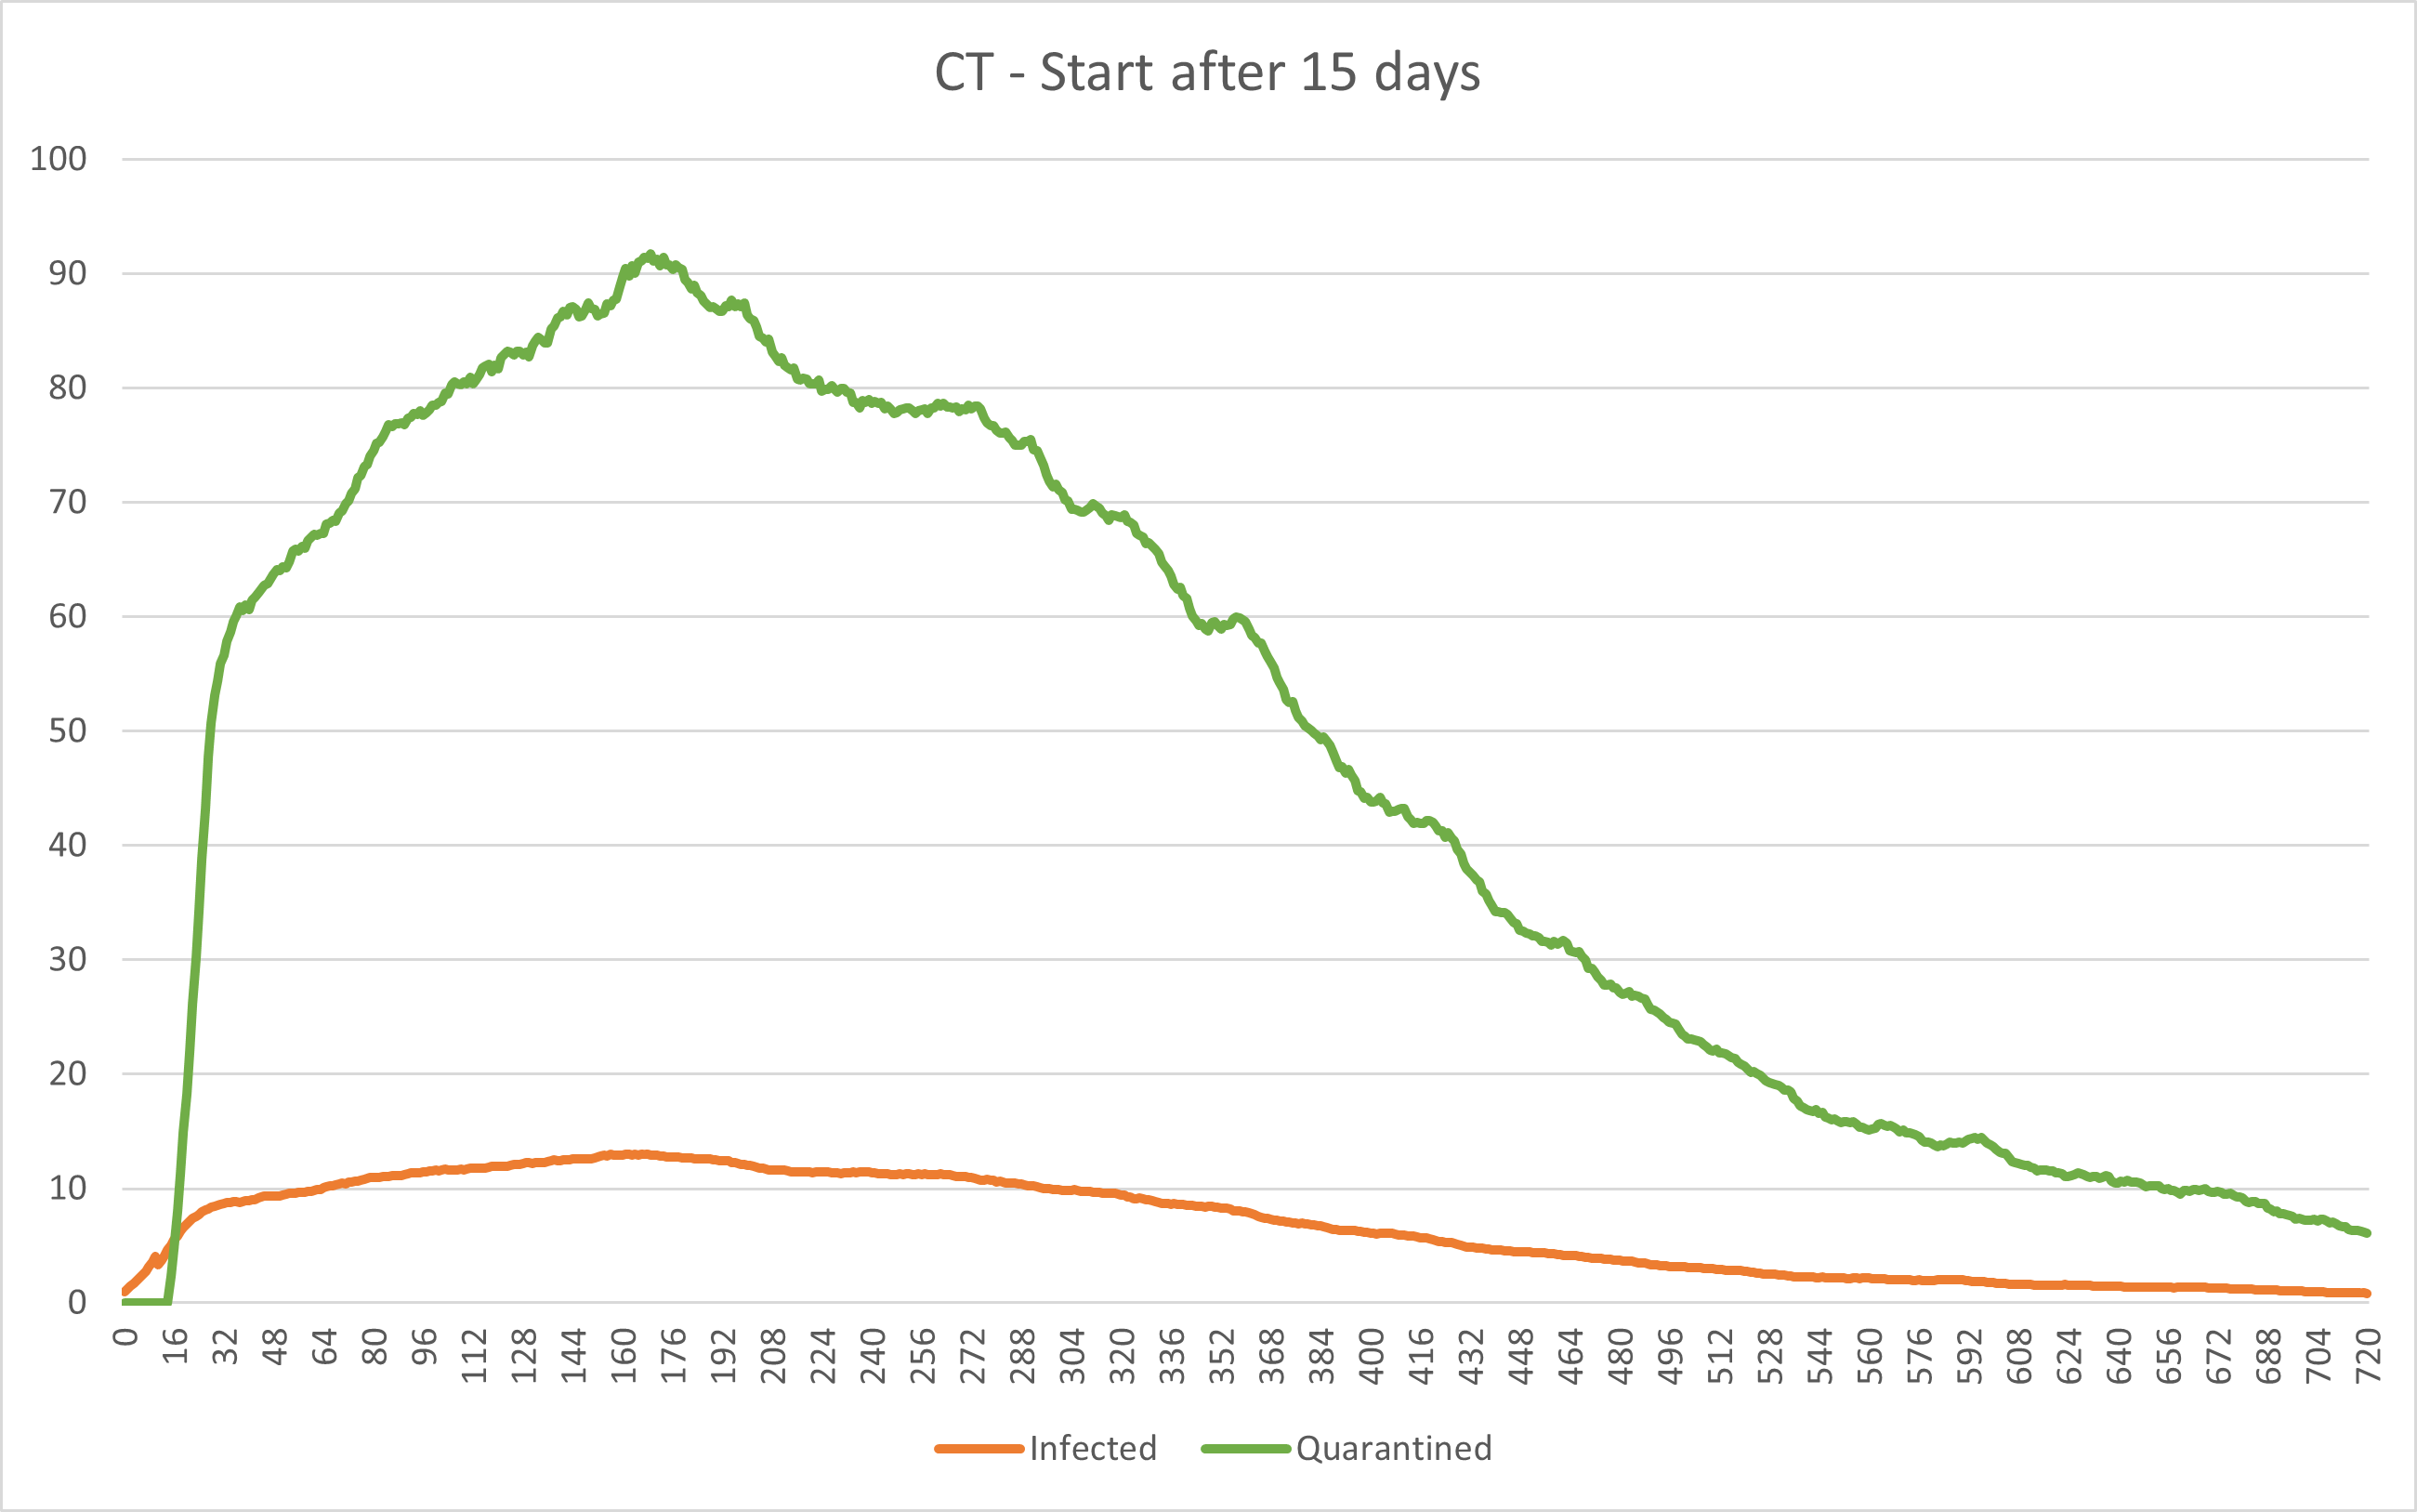
\includegraphics[width=.95\linewidth]{0_billeder/CT15Days.png}
  \caption{Contact tracing starting after 15 days}
  \label{Subfig:CT15}
\end{subfigure}%
\begin{subfigure}{.5\textwidth}
  \centering
  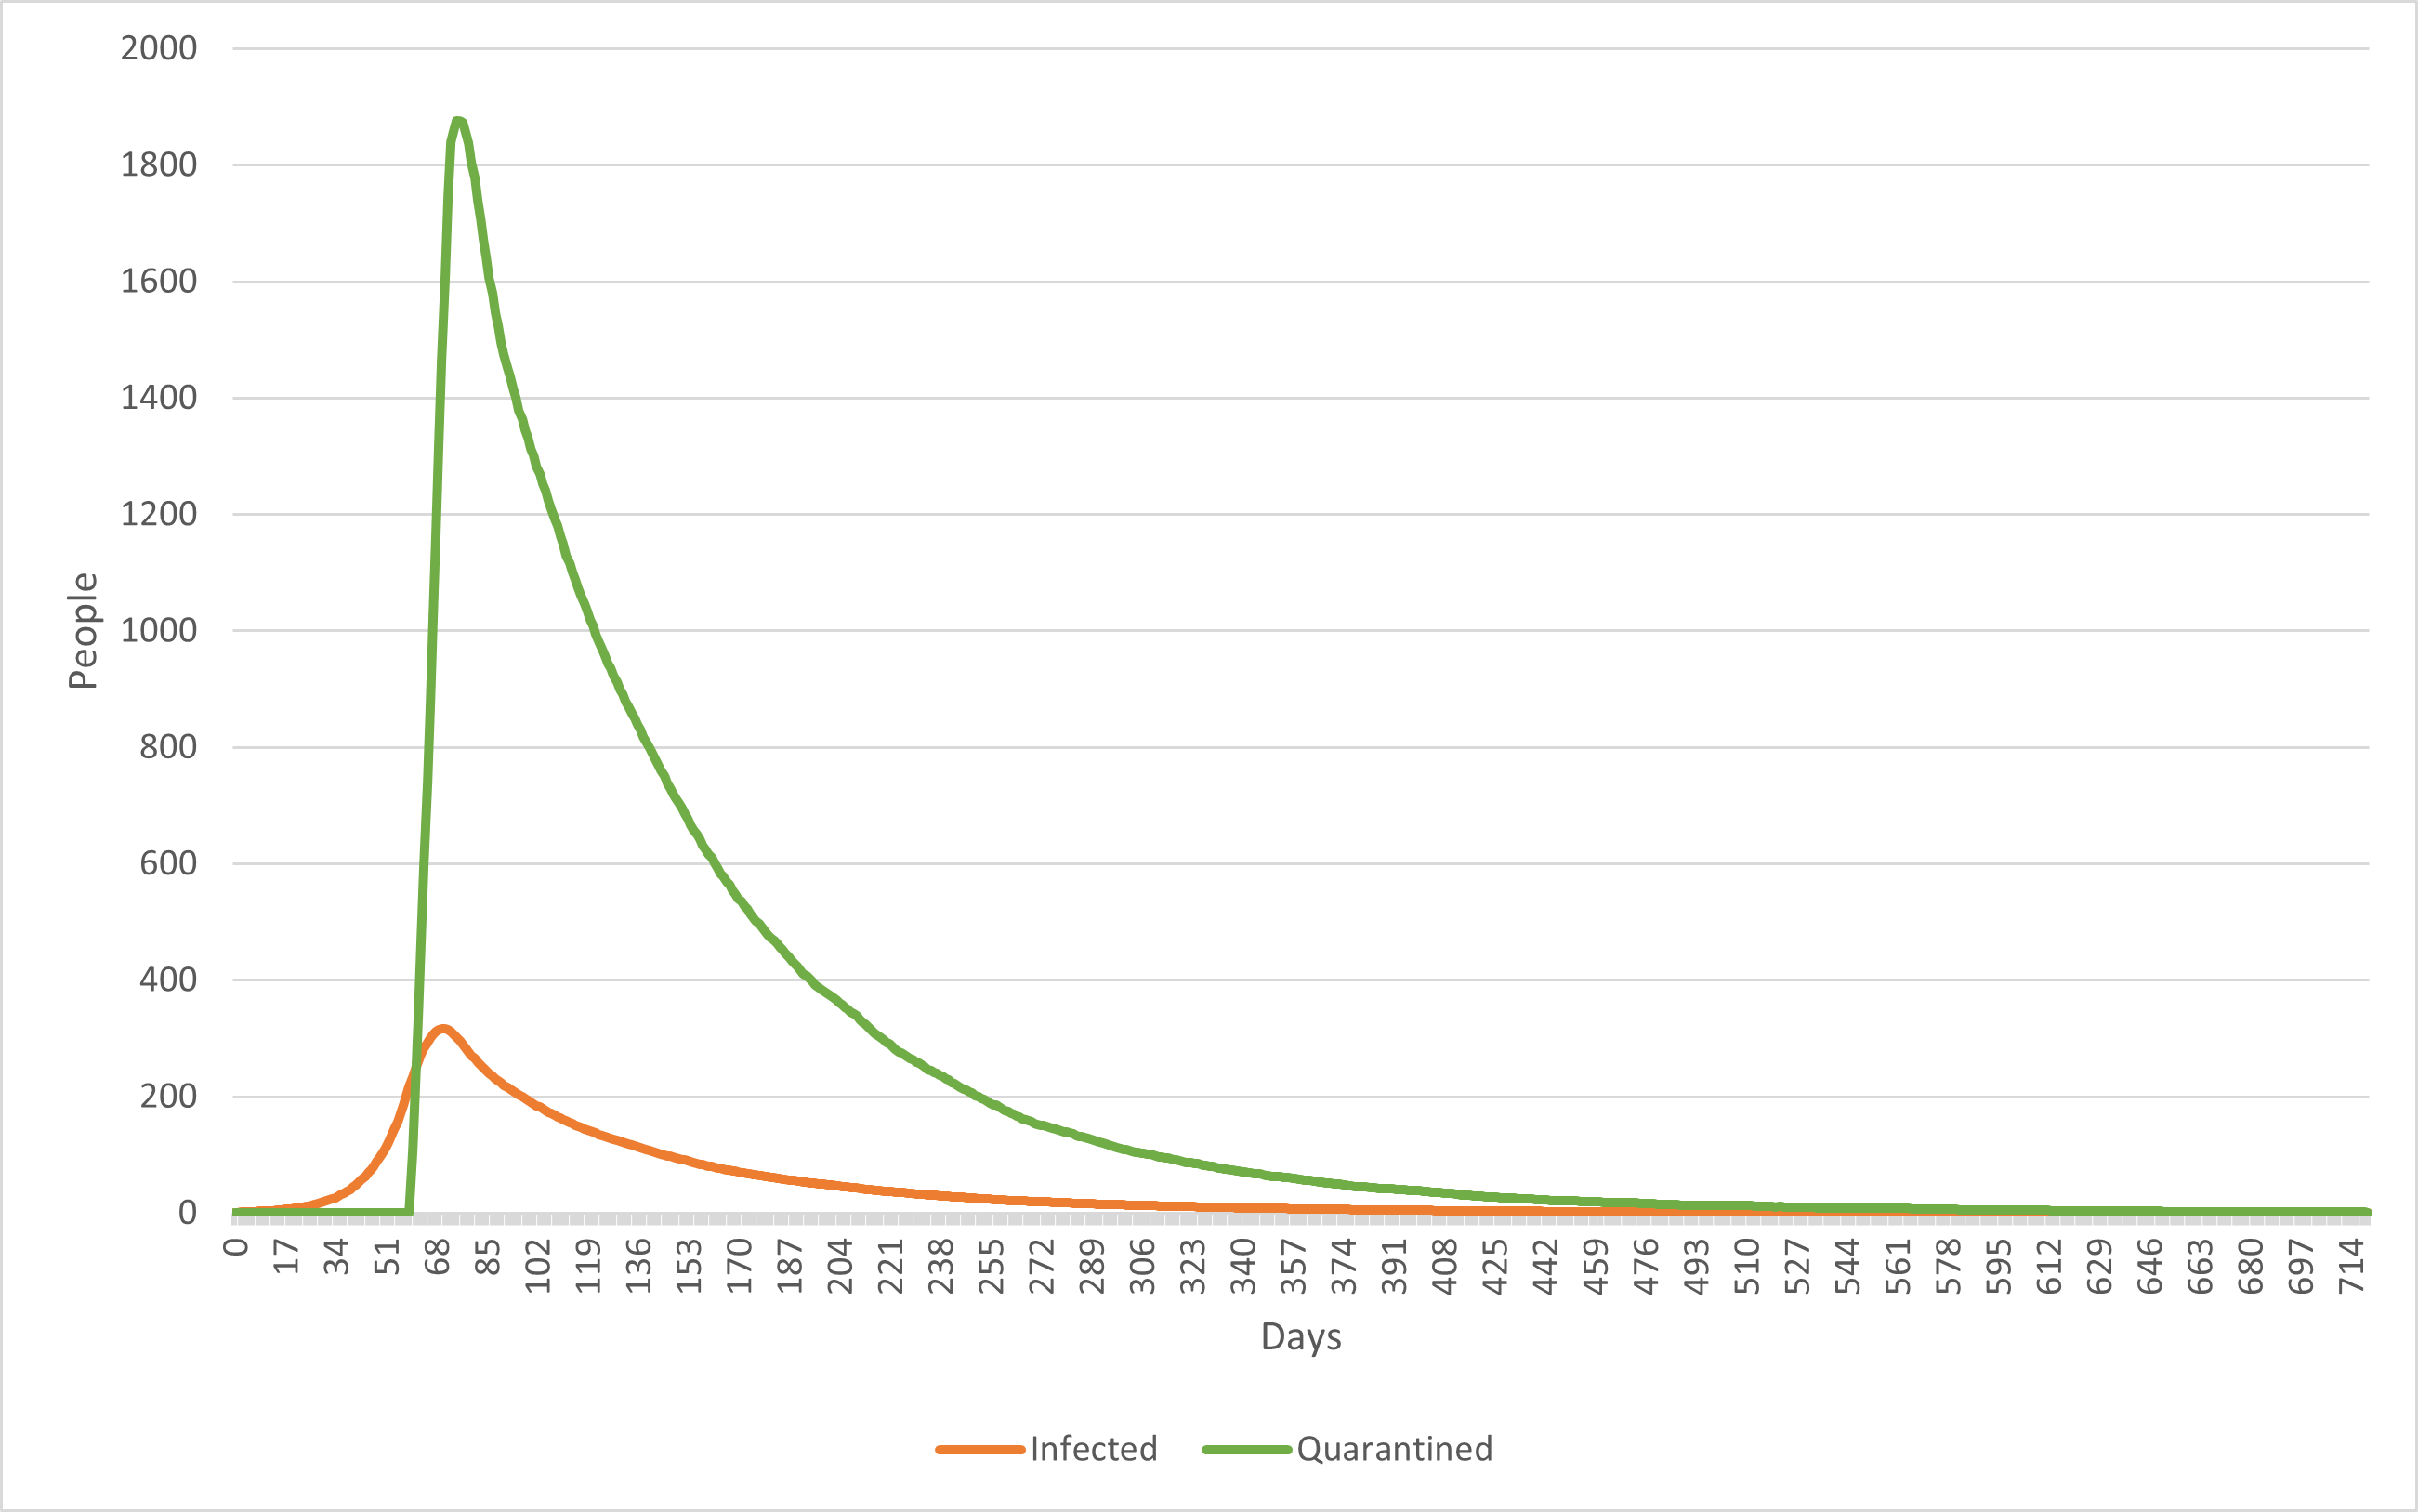
\includegraphics[width=.95\linewidth]{0_billeder/CT60Days.png}
  \caption{Contact tracing starting after 60 days}
  \label{Subfig:CT60}
\end{subfigure}
\caption{Graphs for number of people quarantined and infected plotted against days (Be aware of different proportions on the y-axis)}
\label{fig:CTstart1}
\end{figure}

From these graphs in figure \ref{fig:CTstart1}, it is obvious that tracing contacts in the population has a huge impact on both how many contacts that needs to be traced in total as well as how many people become infected. It should also be noted that our simulation uses a \say{perfect} form of contact tracing, where everybody is at least able to trace 5 of their contacts over the previous 2 days. This is also why we see such a huge spike in the number of people quarantined when we reach the start time, since somewhere between 5-20 times the number of infected (who are not asymptomatic and not in incubation) will be quarantined.

It is also interesting to see that the early start in figure \ref{Subfig:CT15} results in a much more steady number of infected and a slow decline, when it is compared to the much later start on CT in figure \ref{Subfig:CT60}. This indicates that the earlier we start contact tracing, the lower the amount of people who get infected is. Similarly, a substantial lower amount of the population needs to be traced.

\begin{figure}[H]
\centering
\begin{subfigure}{.5\textwidth}
  \centering
  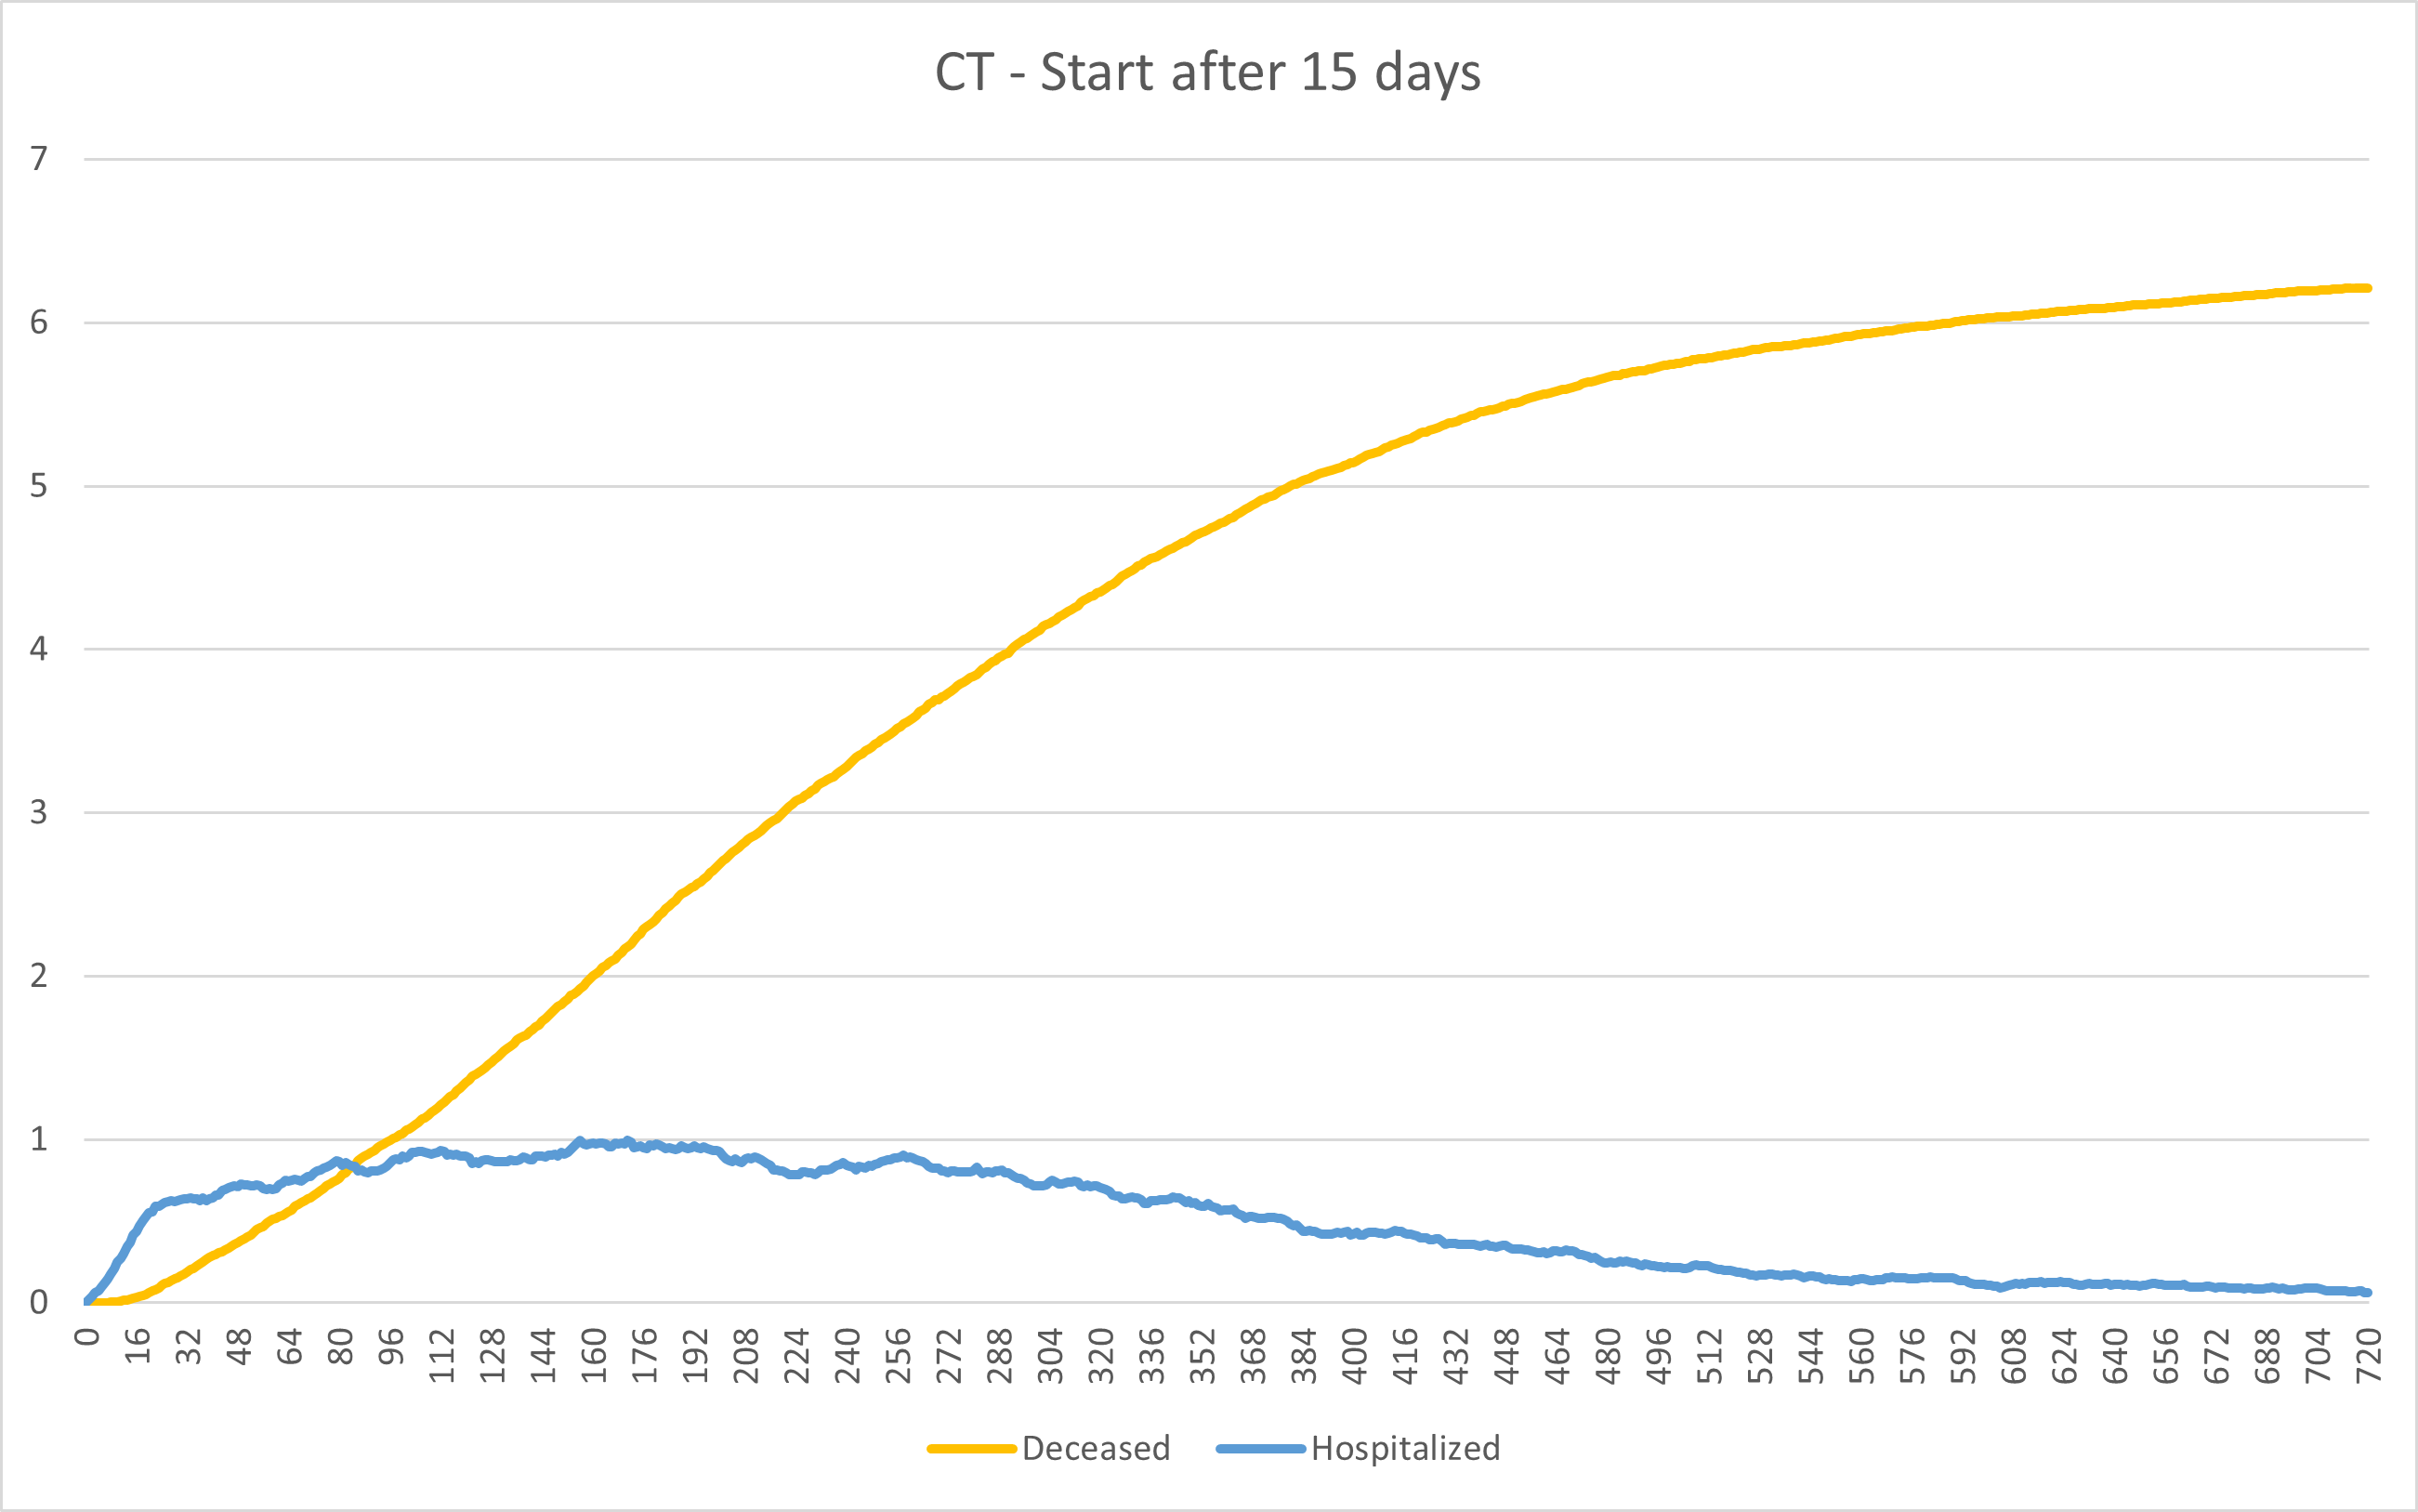
\includegraphics[width=.95\linewidth]{0_billeder/CT15DaysDH.png}
  \caption{Contact tracing starting after 15 days}
  \label{Subfig:CT15DH}
\end{subfigure}%
\begin{subfigure}{.5\textwidth}
  \centering
  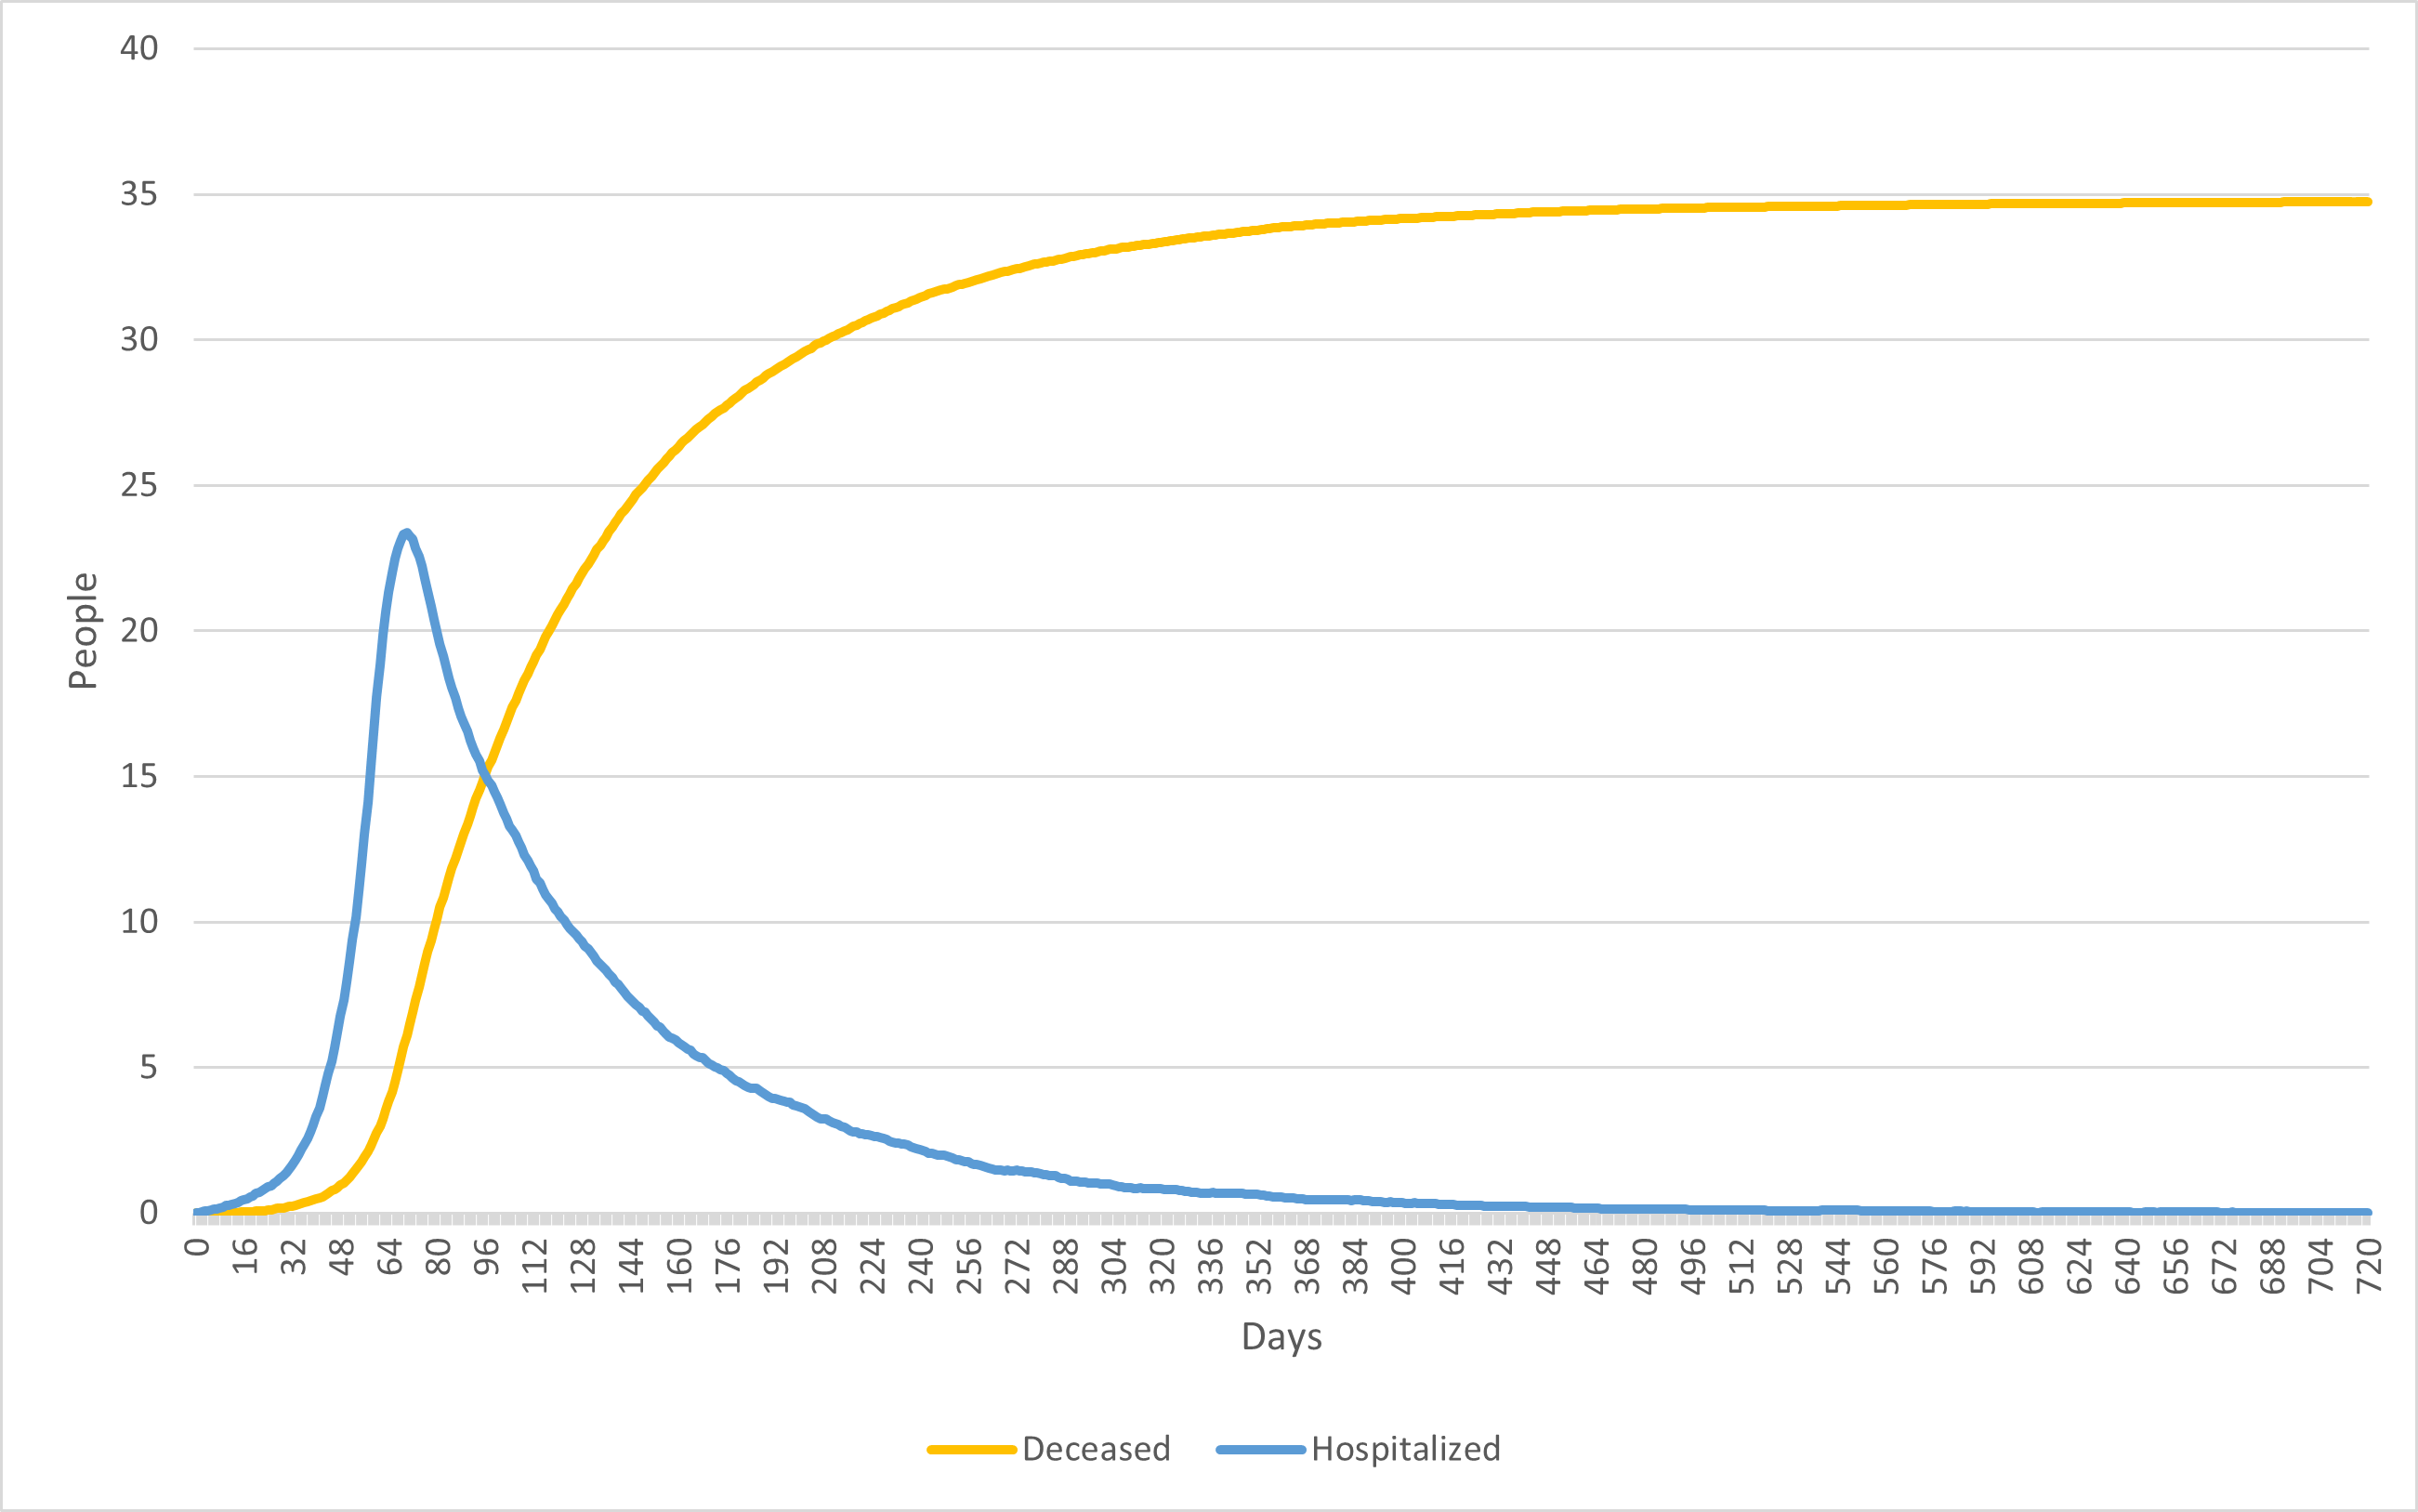
\includegraphics[width=.95\linewidth]{0_billeder/CT60DaysDH.png}
  \caption{Contact tracing starting after 60 days}
  \label{Subfig:CT60DH}
\end{subfigure}
\caption{Graphs for number of people hospitalised and deceased plotted against days (Be aware of different proportions on the y-axis)}
\label{fig:CTstart2}
\end{figure}

Since the starting time had such a notable effect on the number of people who became infected, it also had very big impact on the amount of people who were hospitalised and deceased. This is a trend that should be very similar across all aspects of the simulation that has an effect on the number of infected, since they should directly correlate with the number of hospitalised and deceased.

\subsection{Quarantine Period}
In this section, we are looking at how the quarantine period will affect the number of persons getting infected. We have run a simulation with a quarantine period of 7 day and one with 21 days. The two graphs below show how the two quarantine periods affect the amount people getting infected and are put into quarantine.

\begin{figure}[H]
\centering
\begin{subfigure}{.5\textwidth}
  \centering
  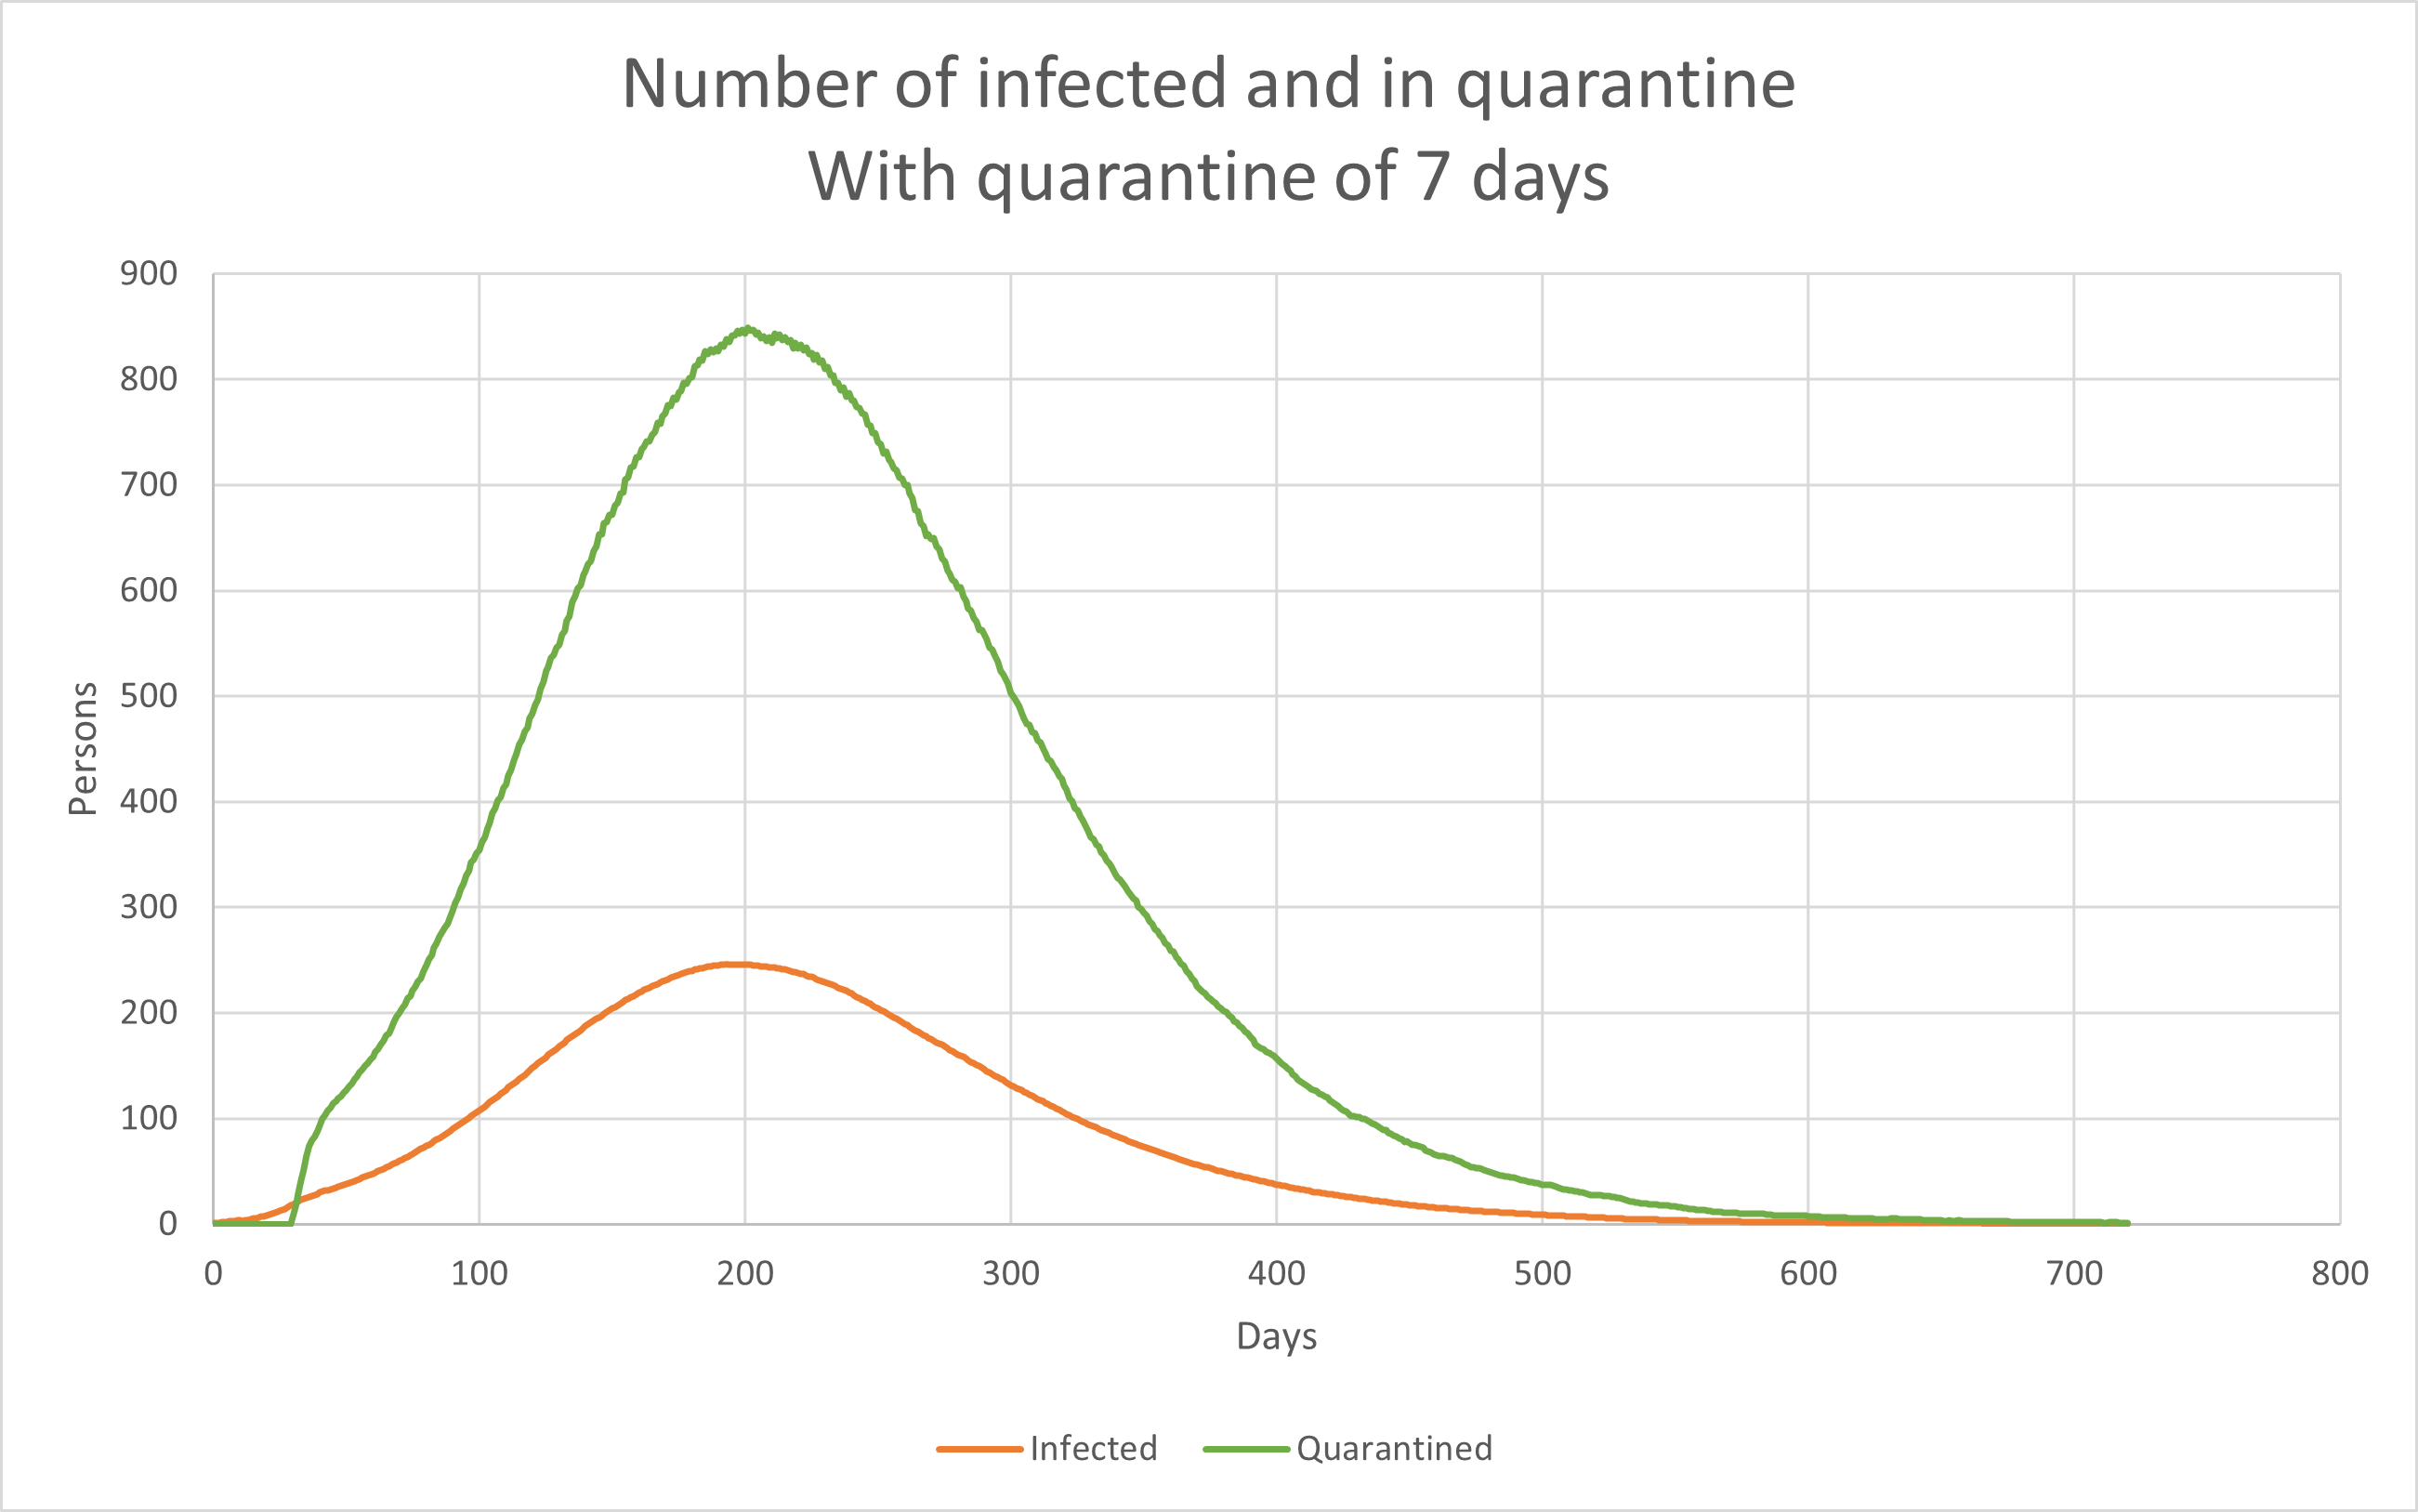
\includegraphics[width=.95\linewidth]{0_billeder/CT_Q_7.png}
  \caption{Quarantined and deceased of 7 days}
  \label{fig:CT_Q_7}
\end{subfigure}%
\begin{subfigure}{.5\textwidth}
  \centering
  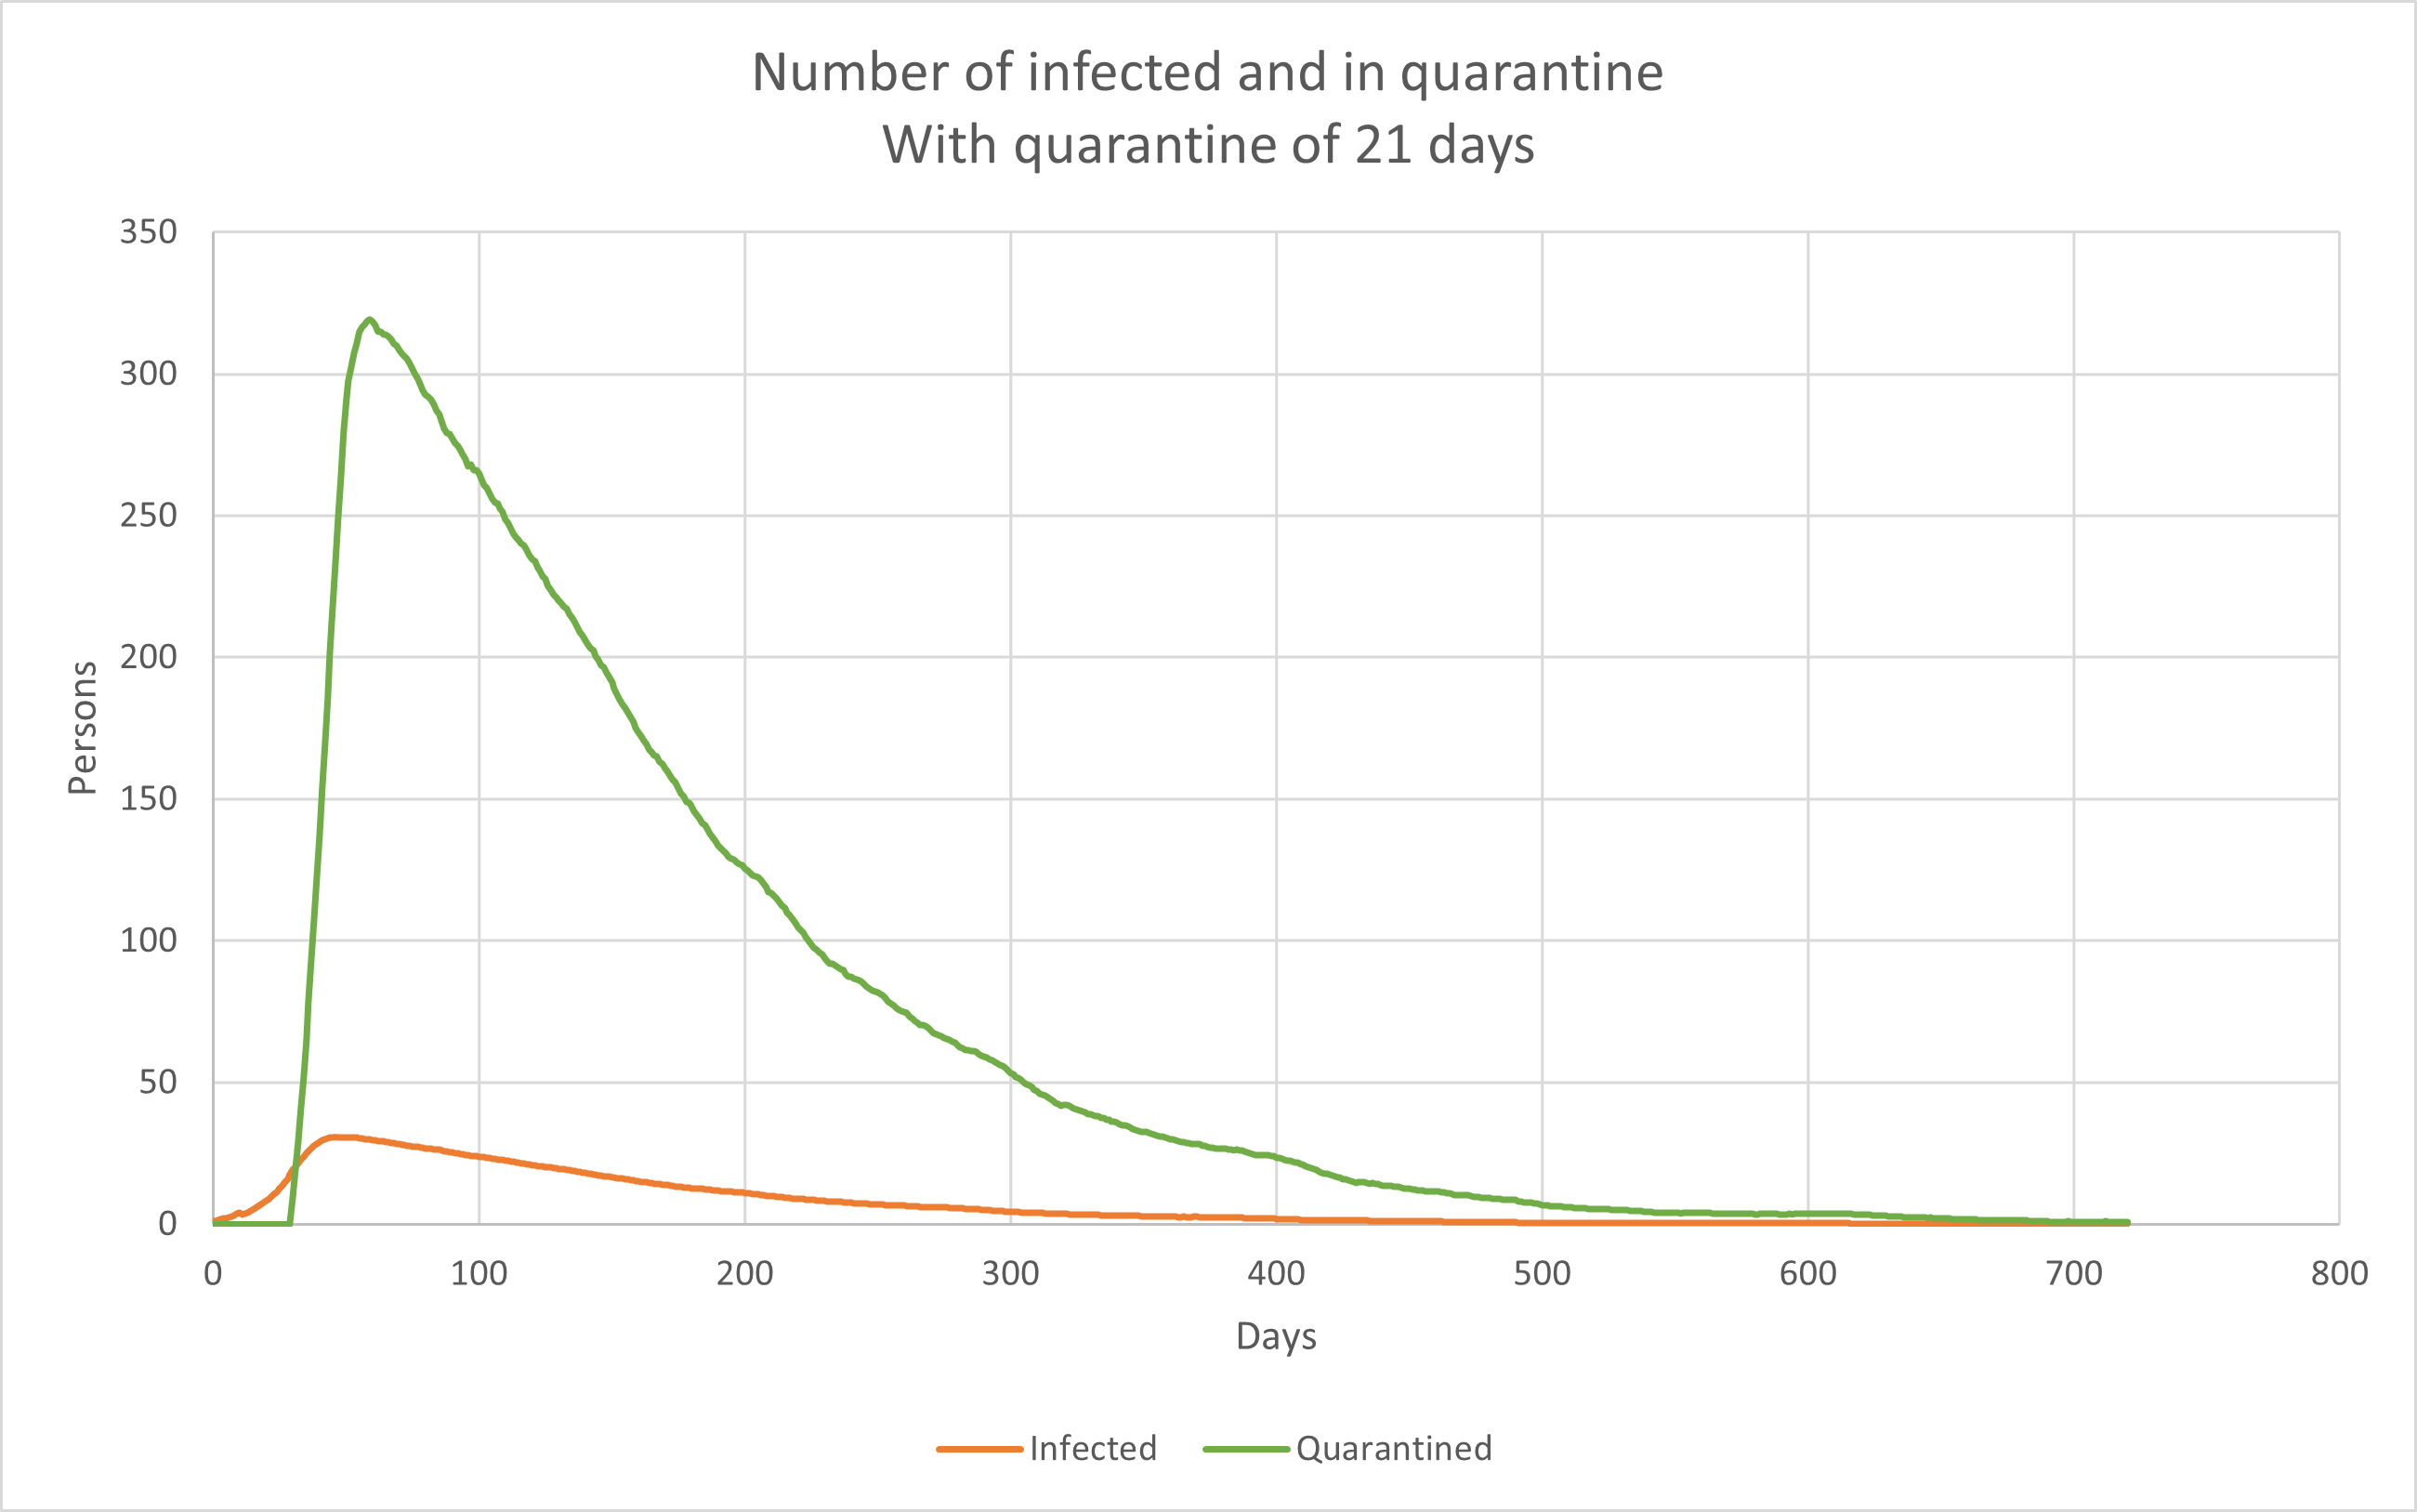
\includegraphics[width=.95\linewidth]{0_billeder/CT_Q_21.png}
  \caption{Quarantined and deceased of 21 days}
  \label{fig:CT_Q_21}
\end{subfigure}
\caption{Comparison between 7 day and 21 day quarantine period with infected and quarantine}
\label{fig:test}
\end{figure}

When the quarantine period is increased, we see that we have a much lower number of infected people per day. With the 7 day quarantine period, we reach the peak of number of infected around day 200 with 230 infected compared to day 50 with a peak around 60 infected for the simulation with 21 quarantine period.

We also see an huge increase in the amount of quarantined people in the 21 day graph, where it takes a couple of days to get 300 people into quarantine, compared to around 60 days to get 300 people into quarantine in the 7 day graph. This of cause leads to a decrease in the amount for people getting deceased shown below.


\begin{figure}[H]
\centering
\begin{subfigure}{.5\textwidth}
  \centering
  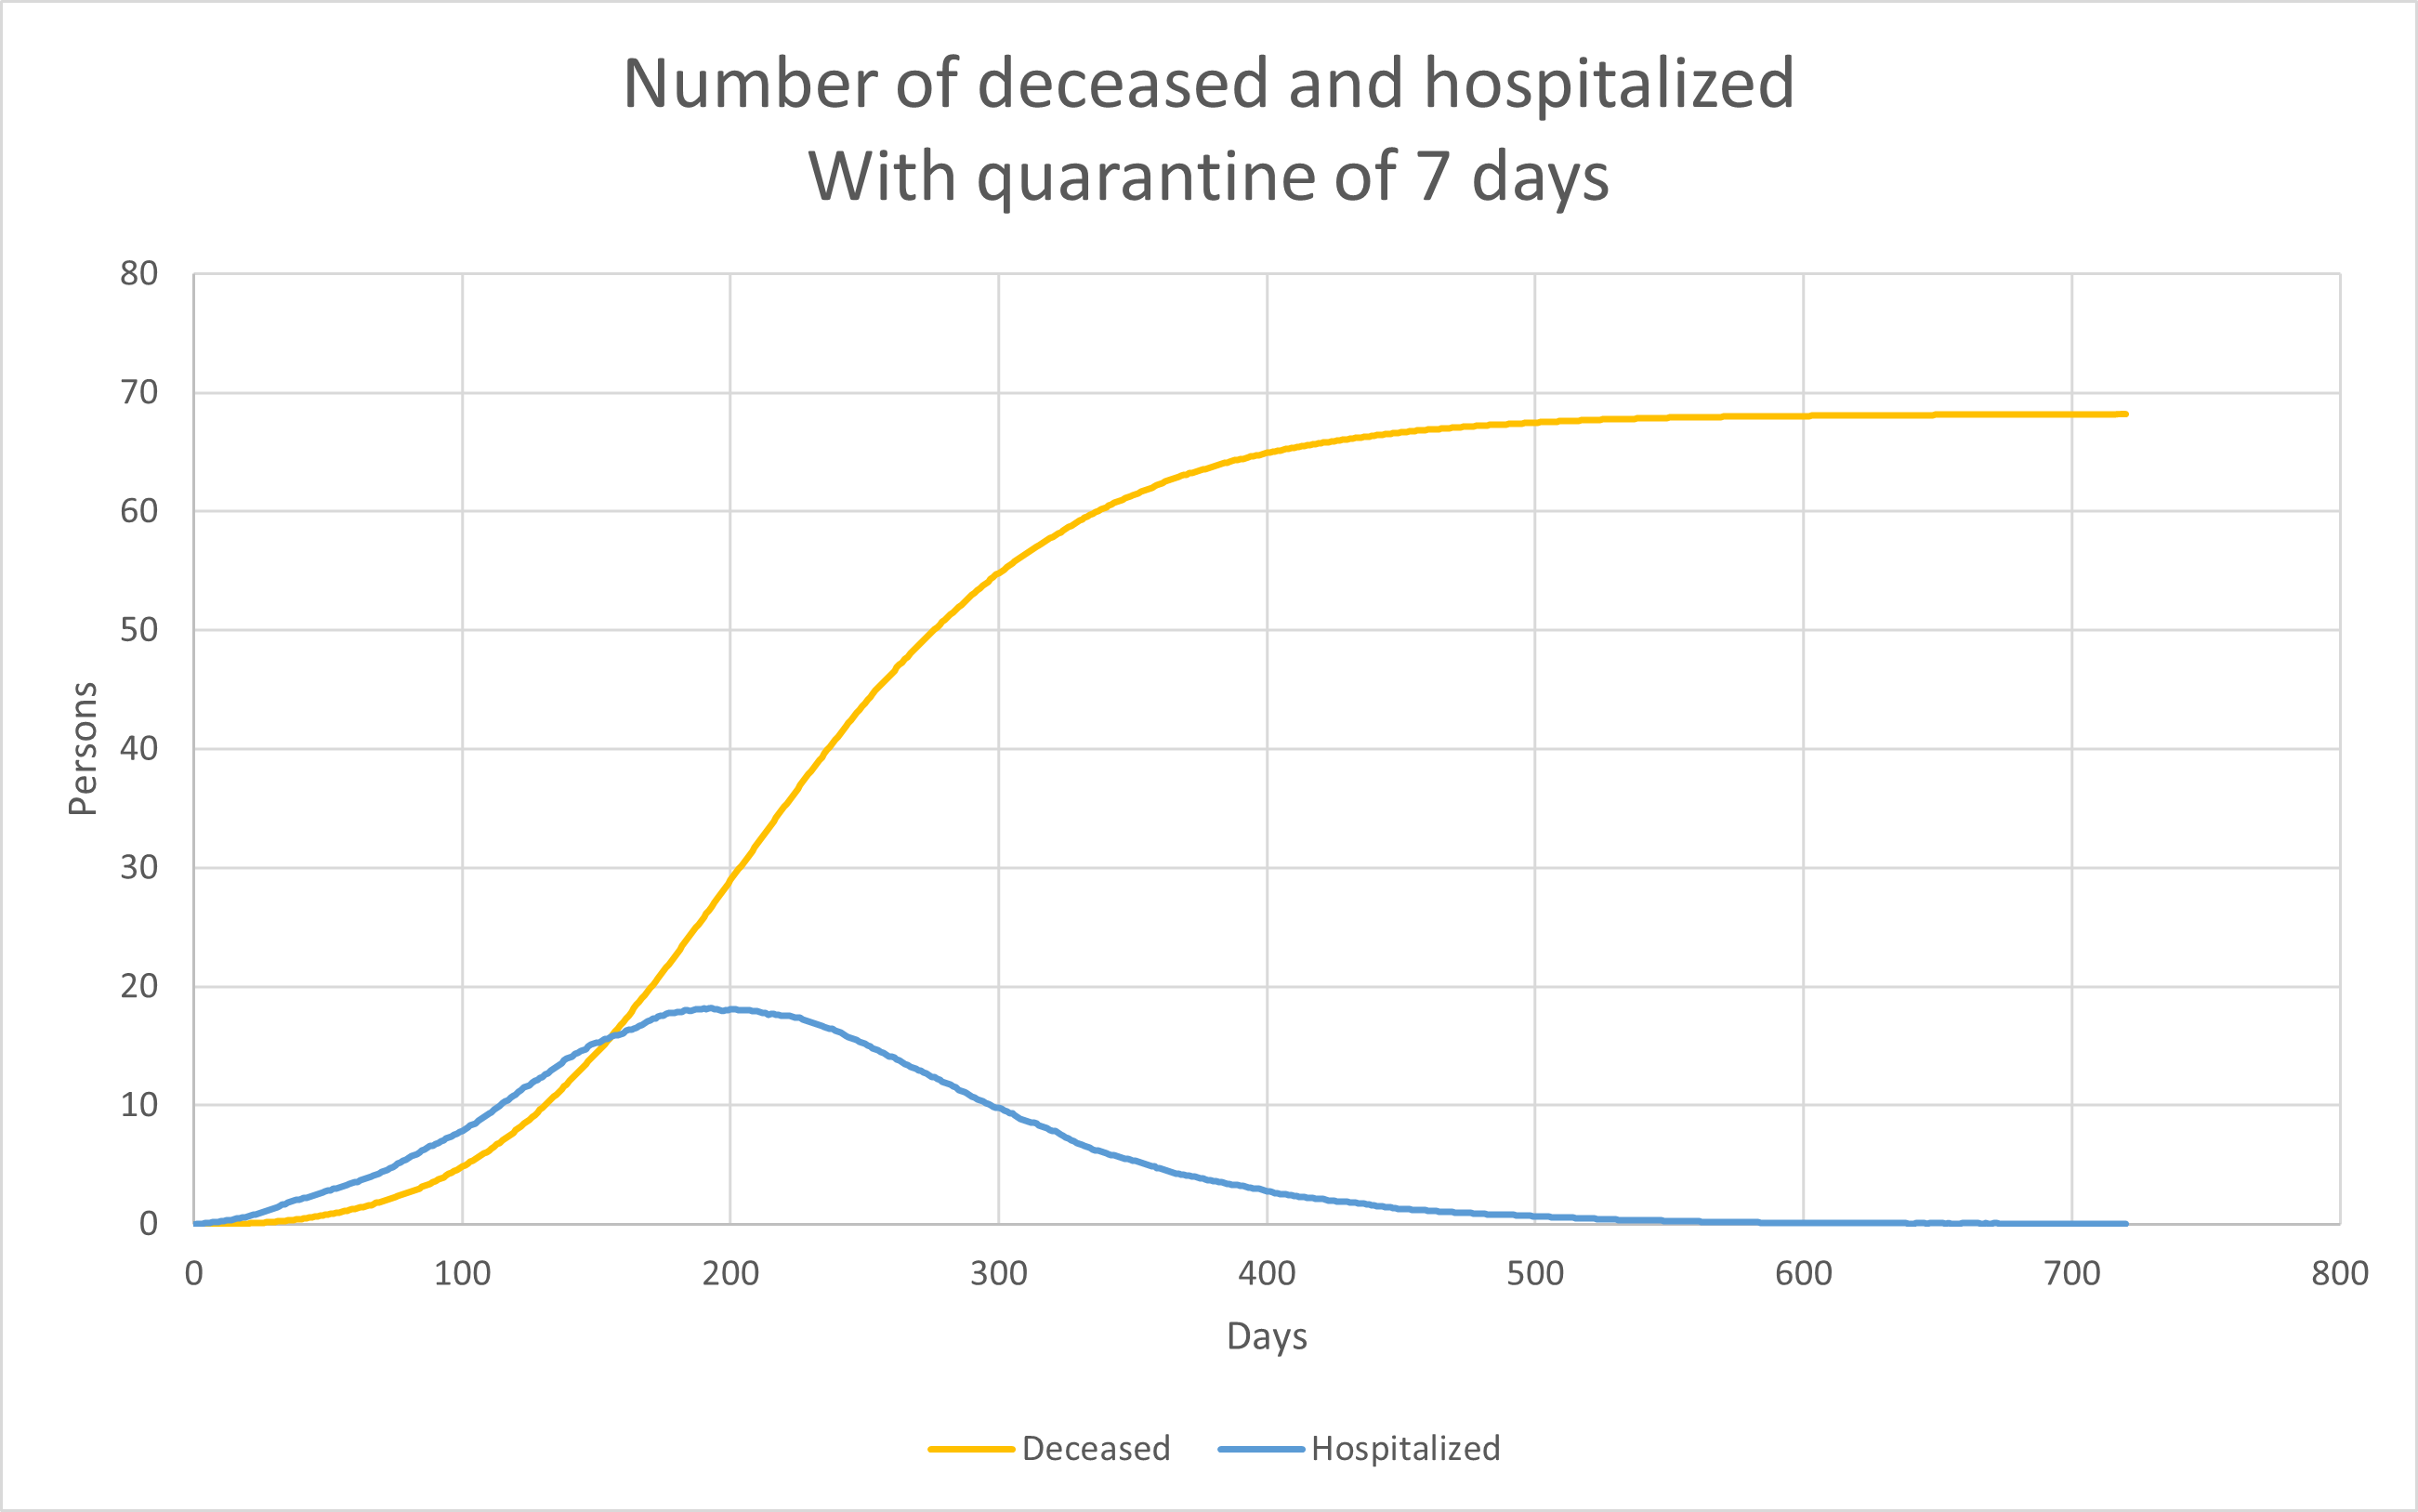
\includegraphics[width=.95\linewidth]{0_billeder/CT_HOS_7.png}
  \caption{Hospitalised and deceased for 7 day quarantine}
  \label{fig:CT_HOS_7}
\end{subfigure}%
\begin{subfigure}{.5\textwidth}
  \centering
  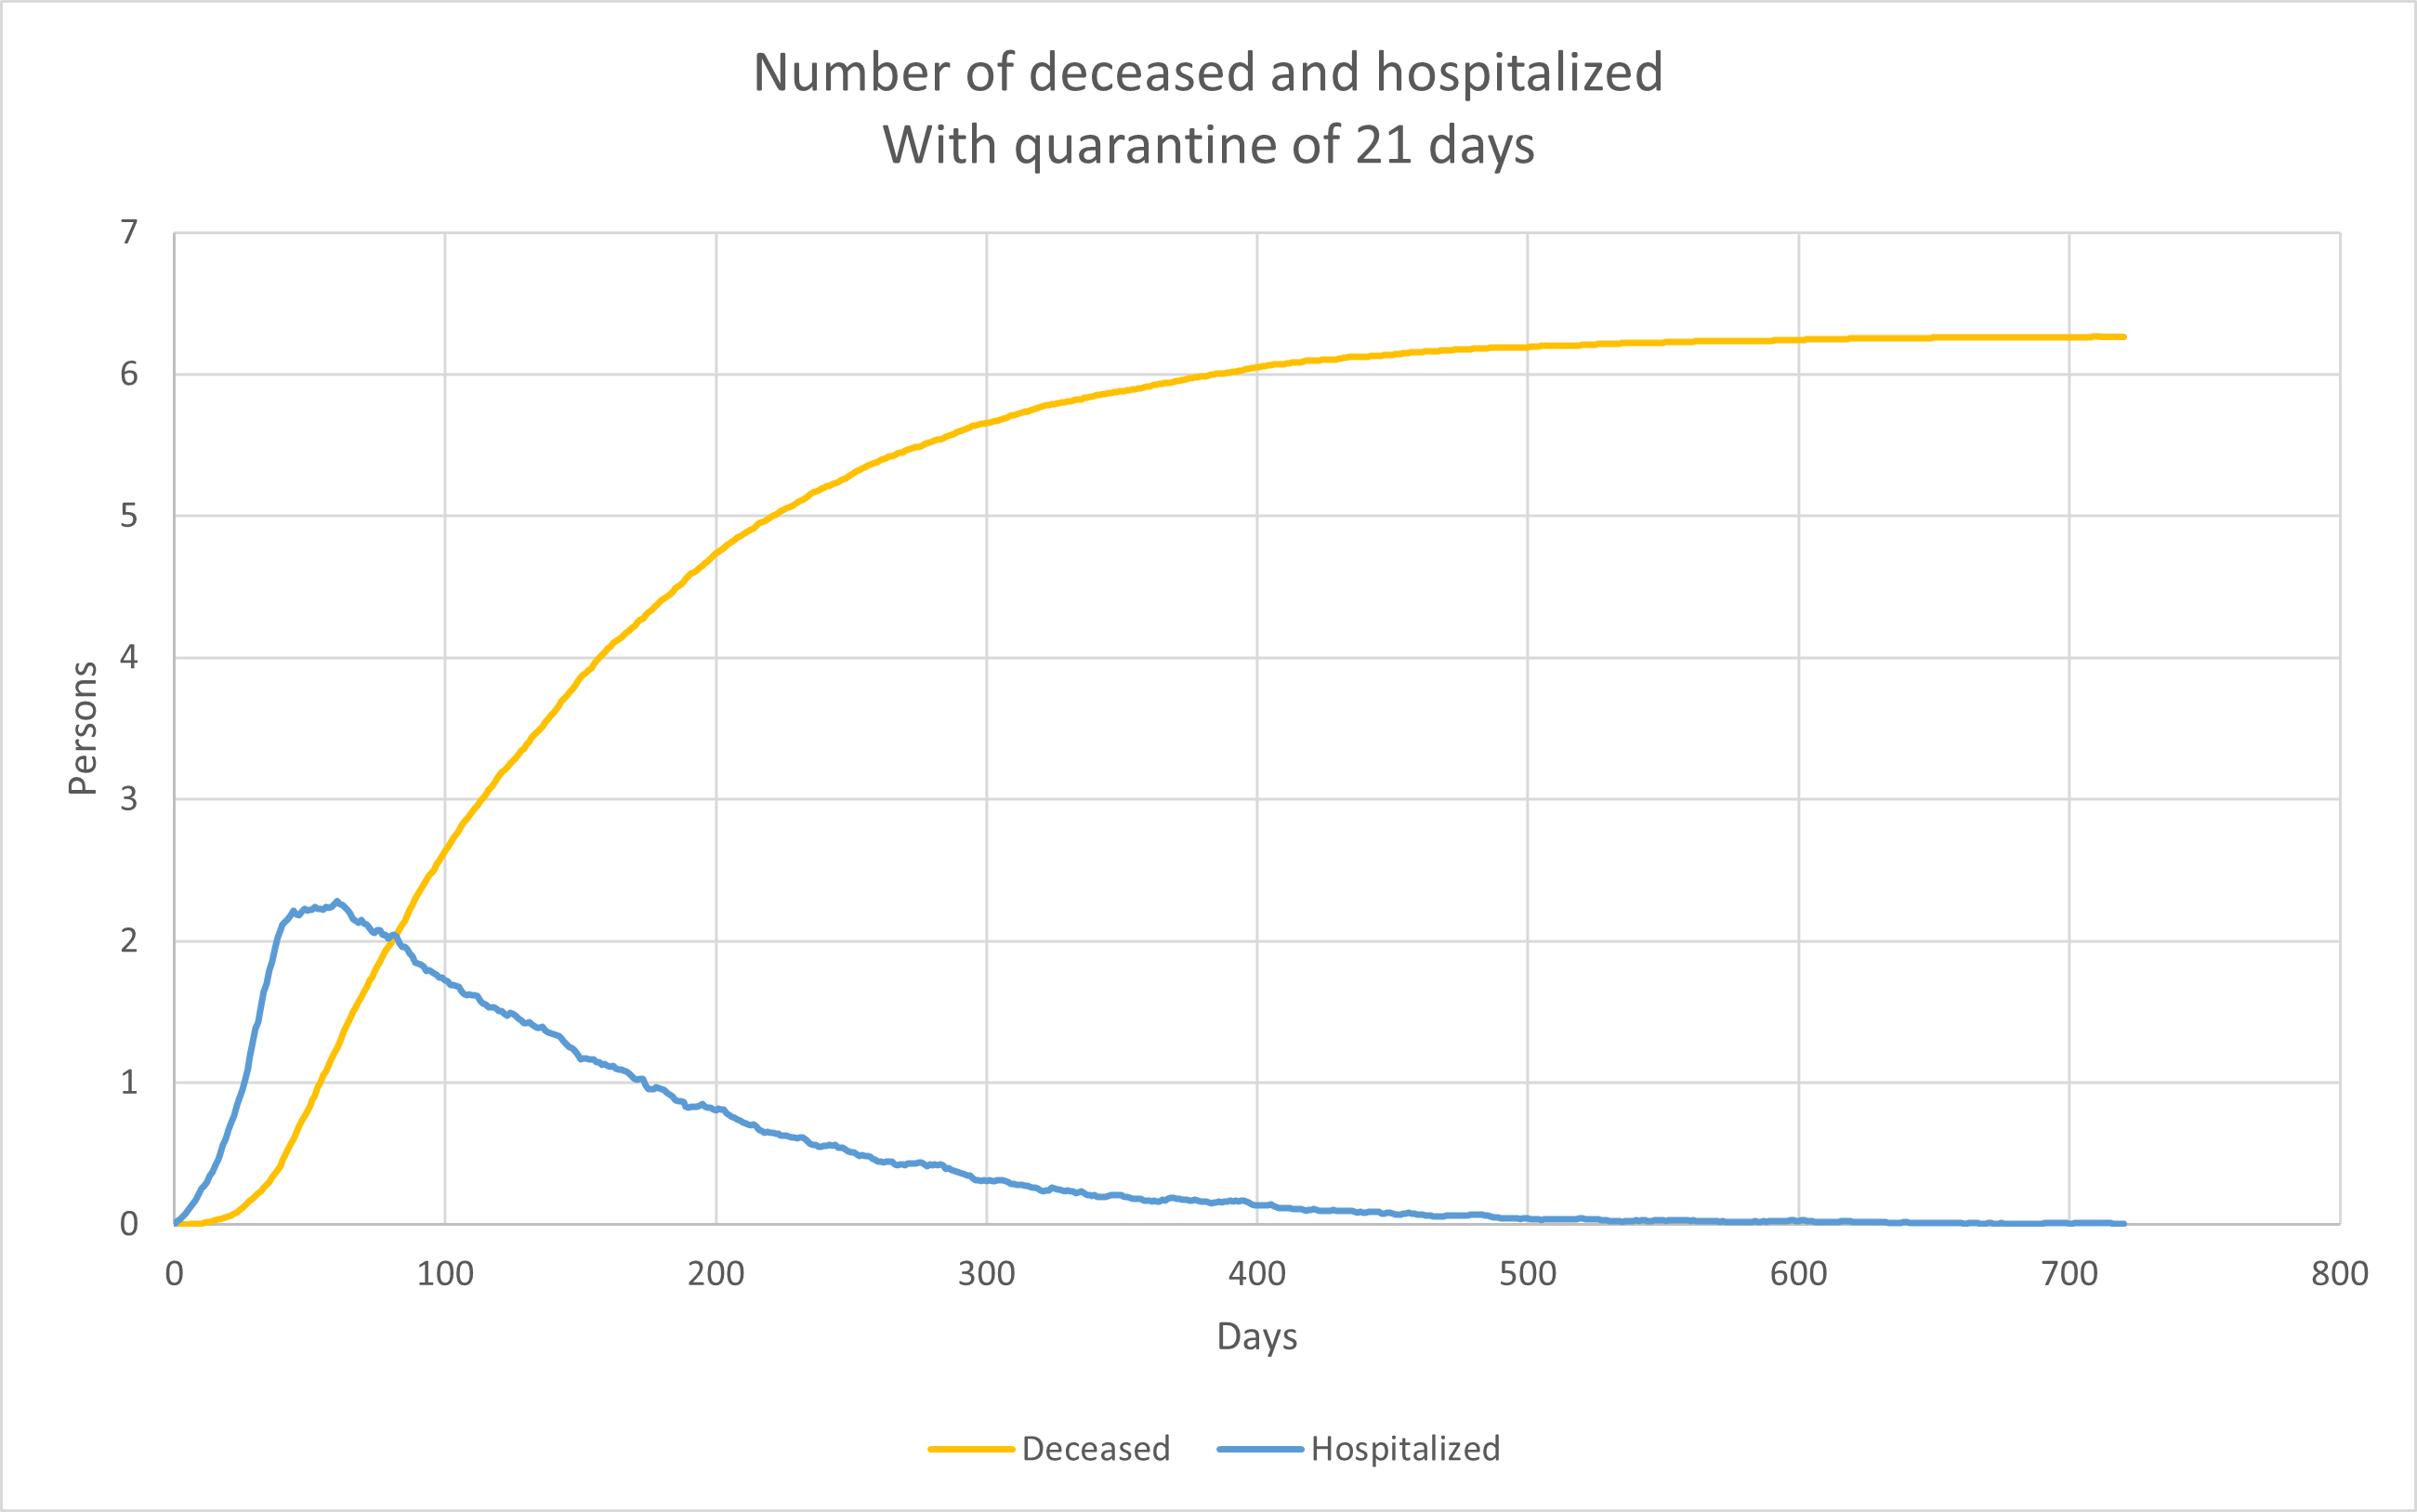
\includegraphics[width=.95\linewidth]{0_billeder/CT_HOS_21.png}
  \caption{Hospitalised and deceased for 21 day quarantine}
  \label{fig:CT_HOS_21}
\end{subfigure}
\caption{Comparison between 7 day and 21 day quarantine period, with deceased and hospitalised}
\label{fig:test}
\end{figure}

Here we see that we have over 10 times the amount of deceased in the graph with 7 day quarantine period compared to 21 days with 69 deceased and 6 deceased respectively. It can also be seen in 21 days graph in the amount of hospitalisations, where it peaks with two hospitalisations and rapidly decreases again when contact tracing begins, compared to 7 day graph where it peaks with 20 hospitalisations.


\subsection{Traceable contacts}

Whether it is possible to trace contacts is imperative for contact tracing to properly work. Therefore, the number of traceable contacts is an important part of the program to do a sensitivity study on. The standard amount of traceable contacts as mentioned earlier is 5-20, we have therefore run our simulation with 0-10 traceable contacts as a lower test and 10-20 traceable contacts as a higher test.

\begin{figure}[H]
\centering
\begin{subfigure}{.5\textwidth}
  \centering
  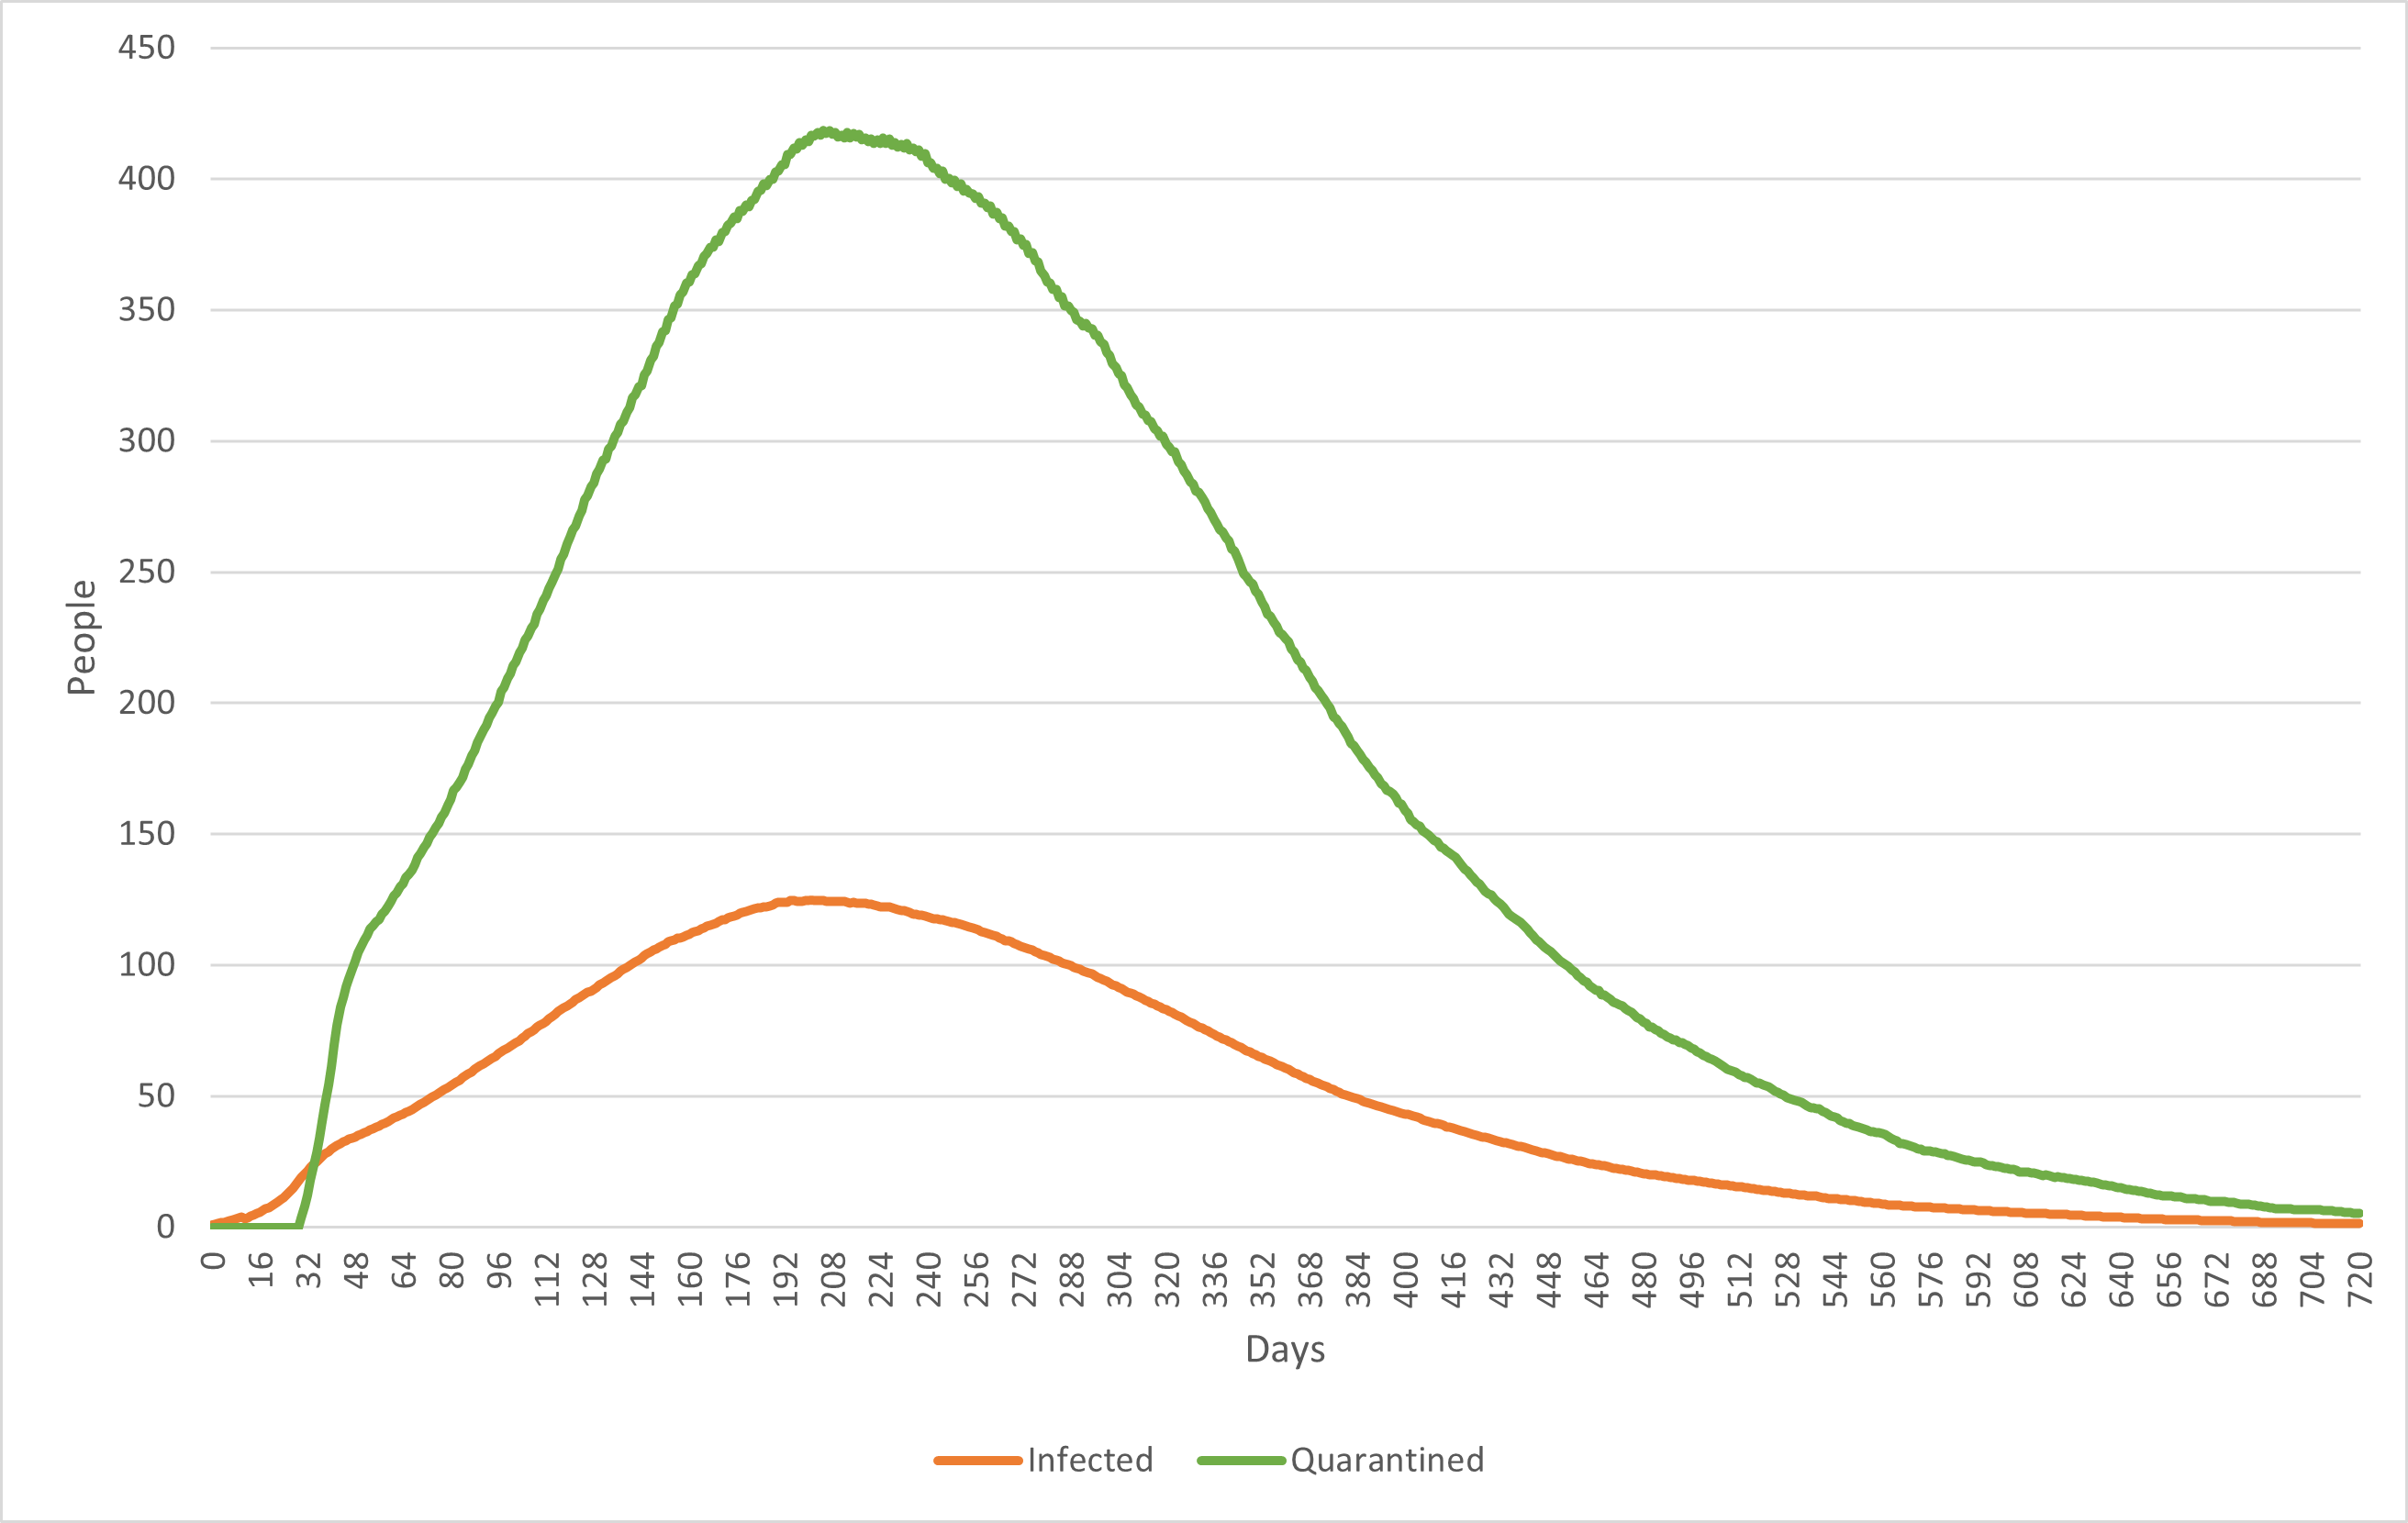
\includegraphics[width=.95\linewidth]{0_billeder/CT-Trace-0-10.png}
  \caption{Contact tracing with 0 to 10 traceable contacts}
  \label{Subfig:CT15DH}
\end{subfigure}%
\begin{subfigure}{.5\textwidth}
  \centering
  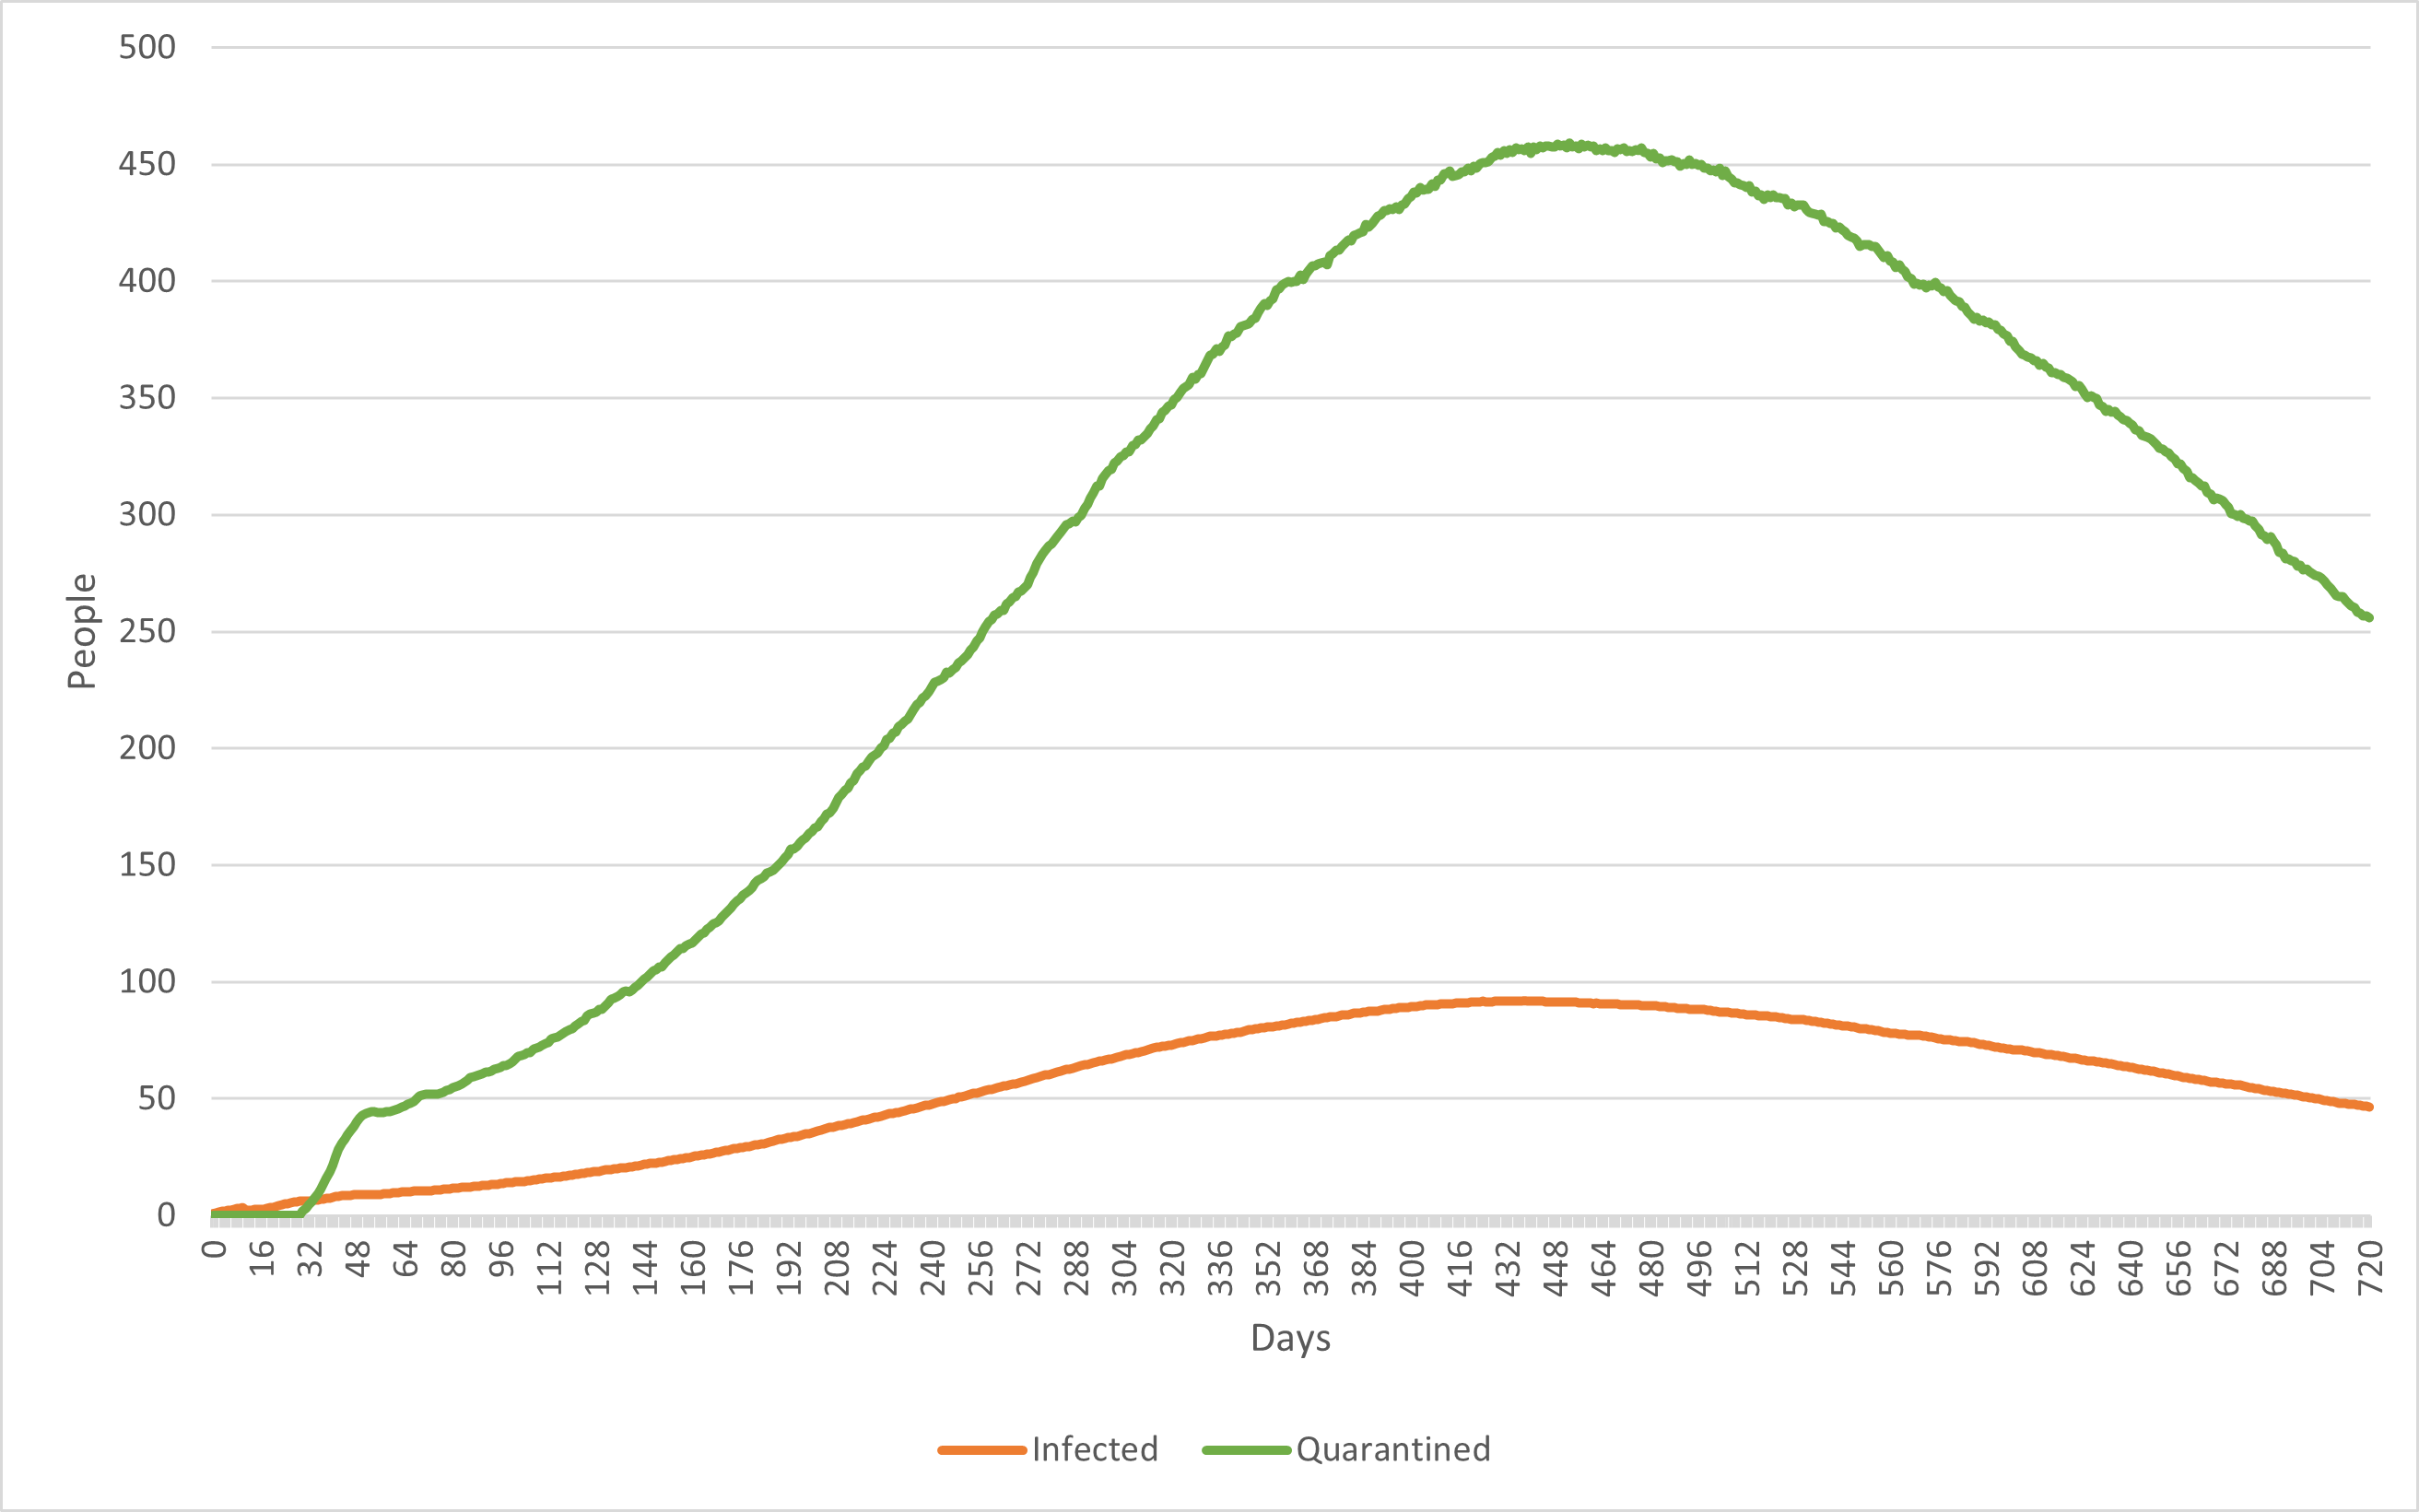
\includegraphics[width=.95\linewidth]{0_billeder/CT-Trace-10-20.png}
  \caption{Contact tracing with 10 to 20 traceable contacts}
  \label{Subfig:CT60DH}
\end{subfigure}
\caption{Graphs for number of people quarantined and infected plotted against days.}
\label{fig:CTstart2}
\end{figure}

As seen in figure \ref{fig:CTstart2}, it is clear that there is a significant difference in the number of potentially traceable contacts. With an increased number of traceable contacts, people are quarantined over a longer period of time. Also, infection peaks later in the time frame and the curve is also lower and softer. Therefore, an increase in traceable contacts would mitigate the spread of the virus.